% arara: xelatex
%% arara: xelatex


% https://koalatea.io/r-knn-regression/
% http://freerangestats.info/blog/2017/04/09/propensity-v-regression
% https://economics.stackexchange.com/questions/45335/what-is-the-difference-between-ate-and-att
% https://kosukeimai.github.io/MatchIt/articles/matching-methods.html


\documentclass[14pt,xcolor=dvipsnames]{beamer}


% !TEX root = om_metrics_14.tex

%\usepackage{epsdice} % dice 1-6 for probability :)

% \usepackage[absolute,overlay]{textpos}

% \usefonttheme[onlymath]{serif}

\usefonttheme{professionalfonts}
% by default beamer changes math fonts for better visibility for projection
% this professionalfonst theme removes this behavior


\usepackage[orientation=portrait,size=custom,width=25.4,height=19.05]{beamerposter}




%25,4 см 19,05 см размеры слайда в powerpoint

\usetheme{metropolis}
\metroset{
  %progressbar=none,
  numbering=none,
  subsectionpage=progressbar,
  block=fill
}

%\usecolortheme{seahorse}

\usepackage{xunicode} % хак для акцентов!
% https://tex.stackexchange.com/questions/28003/

\usepackage{fontspec}
\usepackage{polyglossia}
\setmainlanguage{russian}


% \usepackage{fontawesome5} % removed [fixed]
\setmainfont[Ligatures=TeX]{Myriad Pro}
% \setsansfont{Myriad Pro}




% why do we need \newfontfamily:
% http://tex.stackexchange.com/questions/91507/
\newfontfamily{\cyrillicfonttt}{Myriad Pro}
\newfontfamily{\cyrillicfont}{Myriad Pro}
%\newfontfamily{\cyrillicfontbs}{Myriad Pro}
\newfontfamily{\cyrillicfontsf}{Myriad Pro}


% https://tex.stackexchange.com/questions/175860/why-does-unicode-math-break-the-kerning-of-accents-in-combination-with-amssymb
% "You shouldn't be using amssymb together with unicode-math"
\usepackage{amsmath}
\usepackage{amsthm} % amssymb 


% https://tex.stackexchange.com/questions/483722/
% \usepackage[MnSymbol]{mathspec}  % Includes amsmath.
% \usepackage{mathspec}  % Includes amsmath.
% \setmathsfont(Digits,Latin,Greek,Symbols)[Numbers={Lining,Proportional}]{Latin Modern Math}
% mathspec must be loaded earlier than amsmath



%\usepackage{bm}

% \usepackage{fdsymbol} % \nperp

% \usepackage{unicode-math} % \symbf
% \setmathfont{Latin Modern Math}



\usepackage{centernot}

\usepackage{graphicx}

\usepackage{wrapfig}
% \usepackage{animate} % animations :)
% \usepackage{tikz}
%\usetikzlibrary{shapes.geometric,patterns,positioning,matrix,calc,arrows,shapes,fit,decorations,decorations.pathmorphing}
% \usepackage{pifont}
\usepackage{comment}
\usepackage[font=small,labelfont=bf]{caption}
\captionsetup[figure]{labelformat=empty}
% \includecomment{techno}



%Расположение

\setbeamersize{text margin left=15 mm,text margin right=5mm} 
\setlength{\leftmargini}{38 pt}

%\usepackage{showframe}
%\usepackage{enumitem}
% \setlist{leftmargin=5.5mm}


%Цвета от дирекции

\definecolor{dirblack}{RGB}{58, 58, 58}
\definecolor{dirwhite}{RGB}{245, 245, 245}
\definecolor{dirred}{RGB}{149, 55, 53}
\definecolor{dirblue}{RGB}{0, 90, 171}
\definecolor{dirorange}{RGB}{235, 143, 76}
\definecolor{dirlightblue}{RGB}{75, 172, 198}
\definecolor{dirgreen}{RGB}{155, 187, 89}
\definecolor{dircomment}{RGB}{128, 100, 162}

\setbeamercolor{title separator}{bg=dirlightblue!50, fg=dirblue}

%Цвета блоков

% Голубой блок!
\setbeamercolor{block title}{bg=dirblue!30,fg=dirblack}
\setbeamercolor{block title example}{bg=dirlightblue!50,fg=dirblack}
\setbeamercolor{block body example}{bg=dirlightblue!20,fg=dirblack}

\AtBeginEnvironment{exampleblock}{\setbeamercolor{itemize item}{fg=dirblack}}
%\setbeamertemplate{blocks}[rounded][shadow]

% Набор команд для удобства верстки

% Набор команд для структуризации

%\newcommand{\quest}{\faQuestionCircleO}
%\faPencilSquareO \faPuzzlePiece \faQuestionCircleO  \faIcon*[regular]{file} {\textcolor{dirblue}
%\newcommand{\quest}{\textcolor{dirblue}{\boxed{\textbf{?}}}
%\newcommand{\task}{\faIcon{tasks}}
%\newcommand{\exmpl}{\faPuzzlePiece}
%\newcommand{\dfn}{\faIcon{pen-square}}
%\newcommand{\quest}{\textcolor{dirblue}{\faQuestionCircle[regular]}}
%\newcommand{\acc}[1]{\textcolor{dirred}{#1}}
%\newcommand{\accm}[1]{\textcolor{dirred}{#1}}
%\newcommand{\acct}[1]{\textcolor{dirblue}{#1}}
%\newcommand{\acctm}[1]{\textcolor{dirblue}{#1}}
%\newcommand{\accex}[1]{\textcolor{dirblack}{\bf #1}}
%\newcommand{\accexm}[1]{\textcolor{dirblack}{ \mathbf{#1}}}
%\newcommand{\acclp}[1]{\textcolor{dirorange}{\it #1}}
\newcommand{\todo}[1]{\textcolor{dircomment}{\bf #1}}
%\newcommand{\graylink}[1]{{\fontsize{11}{12}\selectfont \textcolor{gray}{#1}}}
%\newcommand{\figcaption}[1]{{\fontsize{18}{20}\selectfont #1}}


\newcommand{\videotitle}[1]{
    {\fontsize{33}{30}\selectfont \textcolor{dirblue}{\textbf{#1}} }

    %\todo{название видеофрагмента}
}

\newcommand{\lecturetitle}[1]{
  {\fontsize{33}{30}\selectfont \textcolor{dirblue}{\textbf{#1}} }

    %\todo{название лекции}
}





%\newcommand{\spcbig}{\vspace{-10 pt}}
%\newcommand{\spcsmall}{\vspace{-5 pt}}

%\usepackage{listings}
%\lstset{
%xleftmargin=0 pt,
%  basicstyle=\small, 
%  language=Python,
  %tabsize = 2,
%  backgroundcolor=\color{mc!20!white}
%}



%\newcommand{\mypart}[1]{\begin{frame}[standout]{\huge #1}\end{frame}}

\setbeamercolor{background canvas}{bg=}

% frame title setup
\setbeamercolor{frametitle}{bg=,fg=dirblue}
\setbeamertemplate{frametitle}[default][left]

\addtobeamertemplate{frametitle}{\hspace*{0.1 cm}}{\vspace*{0.25cm}}


%Шрифты
\setbeamerfont{frametitle}{family=\rmfamily,series=\bfseries,size={\fontsize{33}{30}}}
\setbeamerfont{framesubtitle}{family=\rmfamily,series=\bfseries,size={\fontsize{26}{20}}}


% удобнее знать номер слайда, чтобы вносить правки!  

\setbeamercolor{footline}{fg=dircomment}
\setbeamerfont{footline}{series=\bfseries, size={\fontsize{12}{14}}}
%\setbeamertemplate{footline}[page number]


\defbeamertemplate{footline}{custom footline}
{%
  \hspace*{\fill}%
  \usebeamercolor[fg]{page number in head/foot}%
  \usebeamerfont{page number in head/foot}%
  page: \insertpagenumber\,/\,\insertpresentationendpage%
  \hspace{20pt}%
  slide: \insertframenumber\,/\,\inserttotalframenumber%
  %\hspace*{\fill}
  \vskip2pt%
}
%\setbeamertemplate{footline}[custom footline]

\usepackage{physics}



% tikz block

\usepackage{pgfplots}
\pgfplotsset{compat=newest}

\usepackage{tikz}
\usetikzlibrary{calc}
\usetikzlibrary{quotes,angles}
\usetikzlibrary{arrows}
\usetikzlibrary{arrows.meta}
\usetikzlibrary{positioning,intersections,decorations.markings}
\usetikzlibrary{patterns}

\usepackage{tkz-euclide} 
%\tikzset{>=latex}

\tikzset{cross/.style={cross out, draw=black, minimum size=2*(#1-\pgflinewidth), inner sep=0pt, outer sep=0pt},
%default radius will be 1pt. 
cross/.default={5pt}}

\colorlet{veca}{red}
\colorlet{vecb}{blue}
\colorlet{vecc}{olive}


\newcommand{\grid}{\draw[color=gray,step=1.0,dotted] (-2.1,-2.1) grid (9.6,6.1)}

% end tikz block

\newcommand{\R}{\mathbb{R}}
\newcommand{\Rot}{\mathrm{R}}
\newcommand{\HH}{\mathrm{H}}
\newcommand{\Id}{\mathrm{I}}
\newcommand{\RR}{\mathbb{R}}
\newcommand{\ZZ}{\mathbb{Z}}
\newcommand{\la}{\lambda}
\let\P\relax
\newcommand{\P}{\mathbb{P}}
\newcommand{\E}{\mathbb{E}}

\newcommand{\cN}{\mathcal{N}}
\newcommand{\qL}{q_{\text{left}}}
\newcommand{\qR}{q_{\text{right}}}



\newcommand{\ba}{\mathbf{a}}
\newcommand{\be}{\mathbf{e}}
\newcommand{\bb}{\mathbf{b}}
\newcommand{\bc}{\mathbf{c}}
\newcommand{\bd}{\mathbf{d}}
\newcommand{\bx}{\mathbf{x}}
\newcommand{\bff}{\mathbf{f}} % \bf is already def
\newcommand{\bv}{\mathbf{v}}
\newcommand{\bzero}{\mathbf{0}}


\DeclareMathOperator{\Var}{Var}
\DeclareMathOperator{\sVar}{sVar}

\DeclareMathOperator{\plim}{plim}


\newcommand{\graylink}[1]{{\fontsize{11}{12}\selectfont \textcolor{gray}{#1}}}
\newcommand{\figcaption}[1]{{\fontsize{18}{20}\selectfont #1}}





\begin{document}


\begin{frame} % название лекции


\lecturetitle{Временные ряды: \\компоненты и наивные модели}

\end{frame}


% !TEX root = ../om_ts_01.tex

\begin{frame} % название фрагмента

\videotitle{Данные и задачи}

\end{frame}



\begin{frame}{Данные и задачи: план}
  \begin{itemize}[<+->]
    \item Временные ряды — тип данных.
    \item Задачи для одного ряда.
    \item Задачи для множества рядов. 
  \end{itemize}

\end{frame}


\begin{frame}{Заговор рептилоидов}

  \alert{Математический анализ:}

  \begin{block}{Последовательность}
    \[
      \frac{1}{2}, \frac{2}{3}, \frac{3}{4}, \frac{4}{5}, \ldots
    \]
  \end{block}
  
  \pause

  \begin{block}{Ряд}
    \[
      \frac{1}{2} + \frac{1}{4} + \frac{1}{8} +  \frac{1}{16} + \ldots
    \]
  \end{block}
  
  \pause

  Временные ряды — \alert{не ряды!}
\end{frame}
  



\begin{frame}{Что такое временной ряд?}

\begin{block}{Временной ряд}
Последовательность наблюдений, упорядоченных во времени. 
\[
0, 0, 5, 7, 102, 53, 23. 
\]
\end{block}

\pause
\begin{block}{Временной ряд}
Последовательность случайных величин, упорядоченных во времени. 
\[
y_1, y_2, y_3, y_4, \ldots, y_T.
\]
\end{block}
  

\end{frame}


\begin{frame}{Задачи для одного ряда}

\begin{itemize}[<+->]
  \item Спрогнозировать следующие значения.
  \item Восстановить пропущенные значения в середине ряда.
  \item Восстановить отдельные наблюдения по агрегированным.
  \item Обнаружить момент разладки.
  \item Выделить составляющие ряда. 
  \item \ldots 
\end{itemize}

\end{frame}


\begin{frame}{Прогнозируем}

  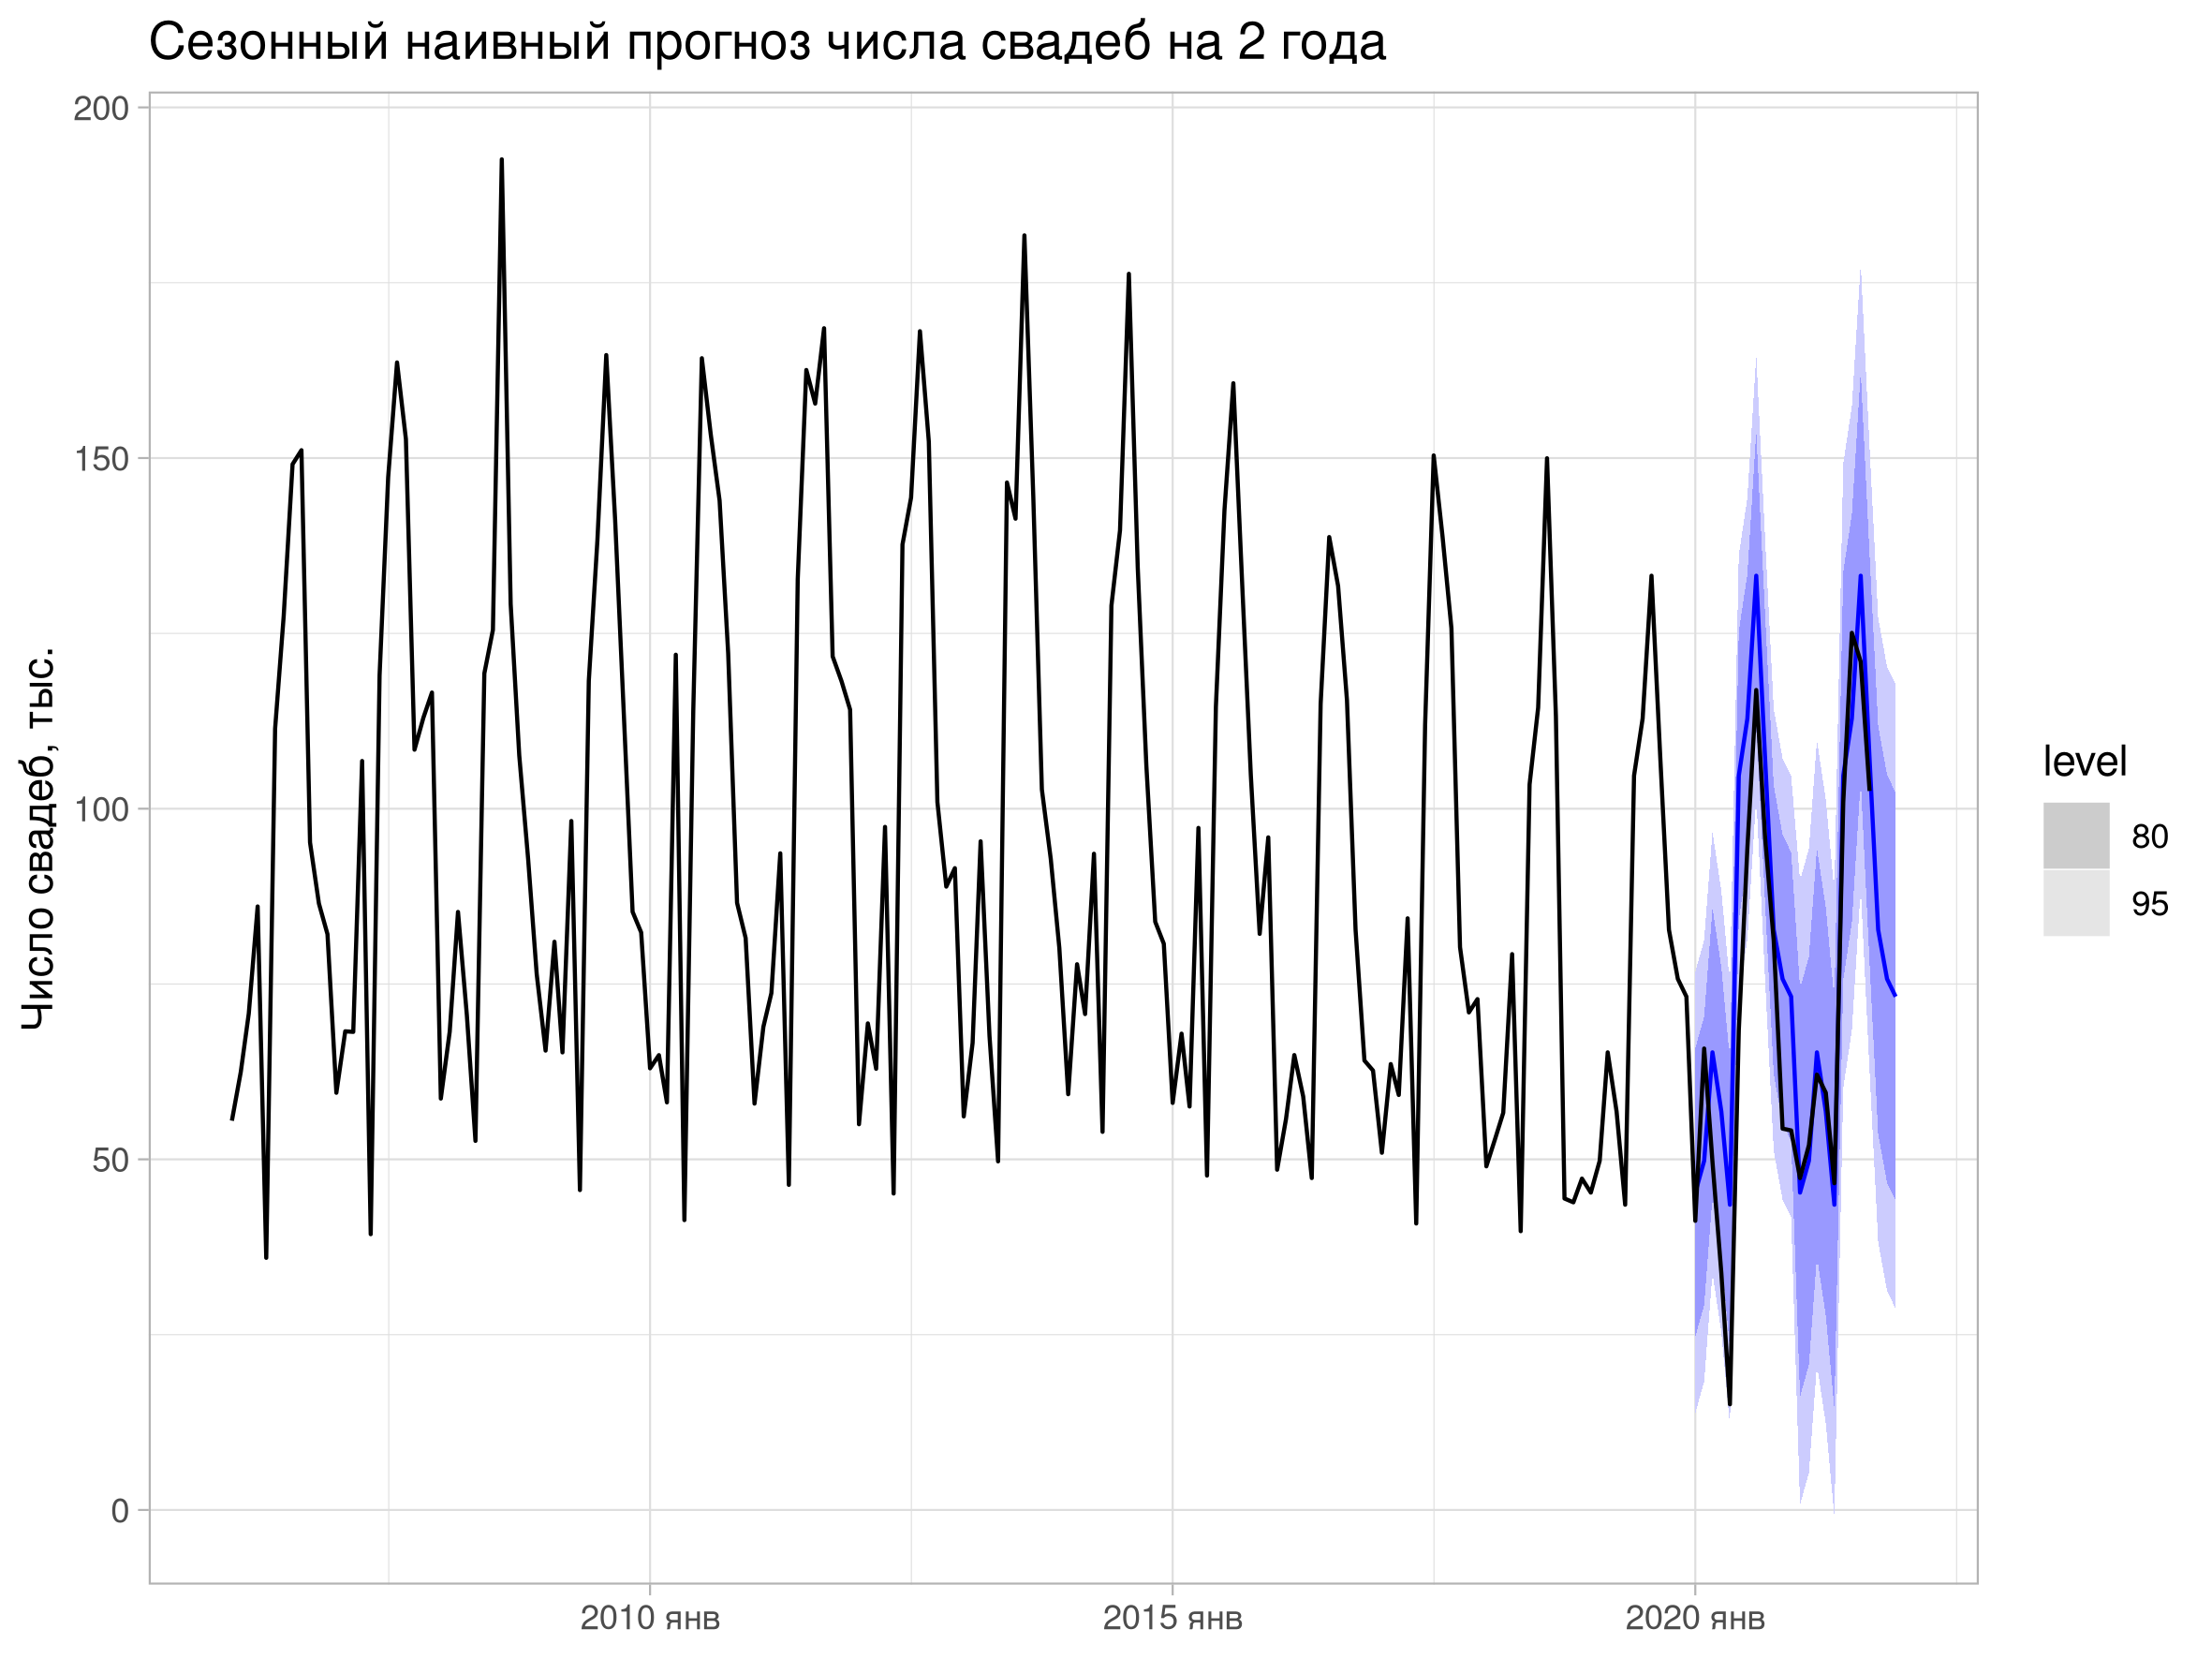
\includegraphics[width=\textwidth]{pictures/om_ts_01-017.png}

\end{frame}


\begin{frame}{Задачи для множества ряда}

  \begin{itemize}[<+->]
    \item Использовать дополнительные ряды при изучении целевого ряда.
    \item Понять, связаны ли ряды между собой.
    \item Измерить причинно-следственные связи.
    \item Классифицировать новый ряд в один из существующих классов.
    \item Понять, какие ряды близки к друг другу.
    \item Кластеризовать ряды на неизвестное множество кластеров.
    \item \ldots
  \end{itemize}
  
\end{frame}
  
\begin{frame}{Измеряем близость рядов}

  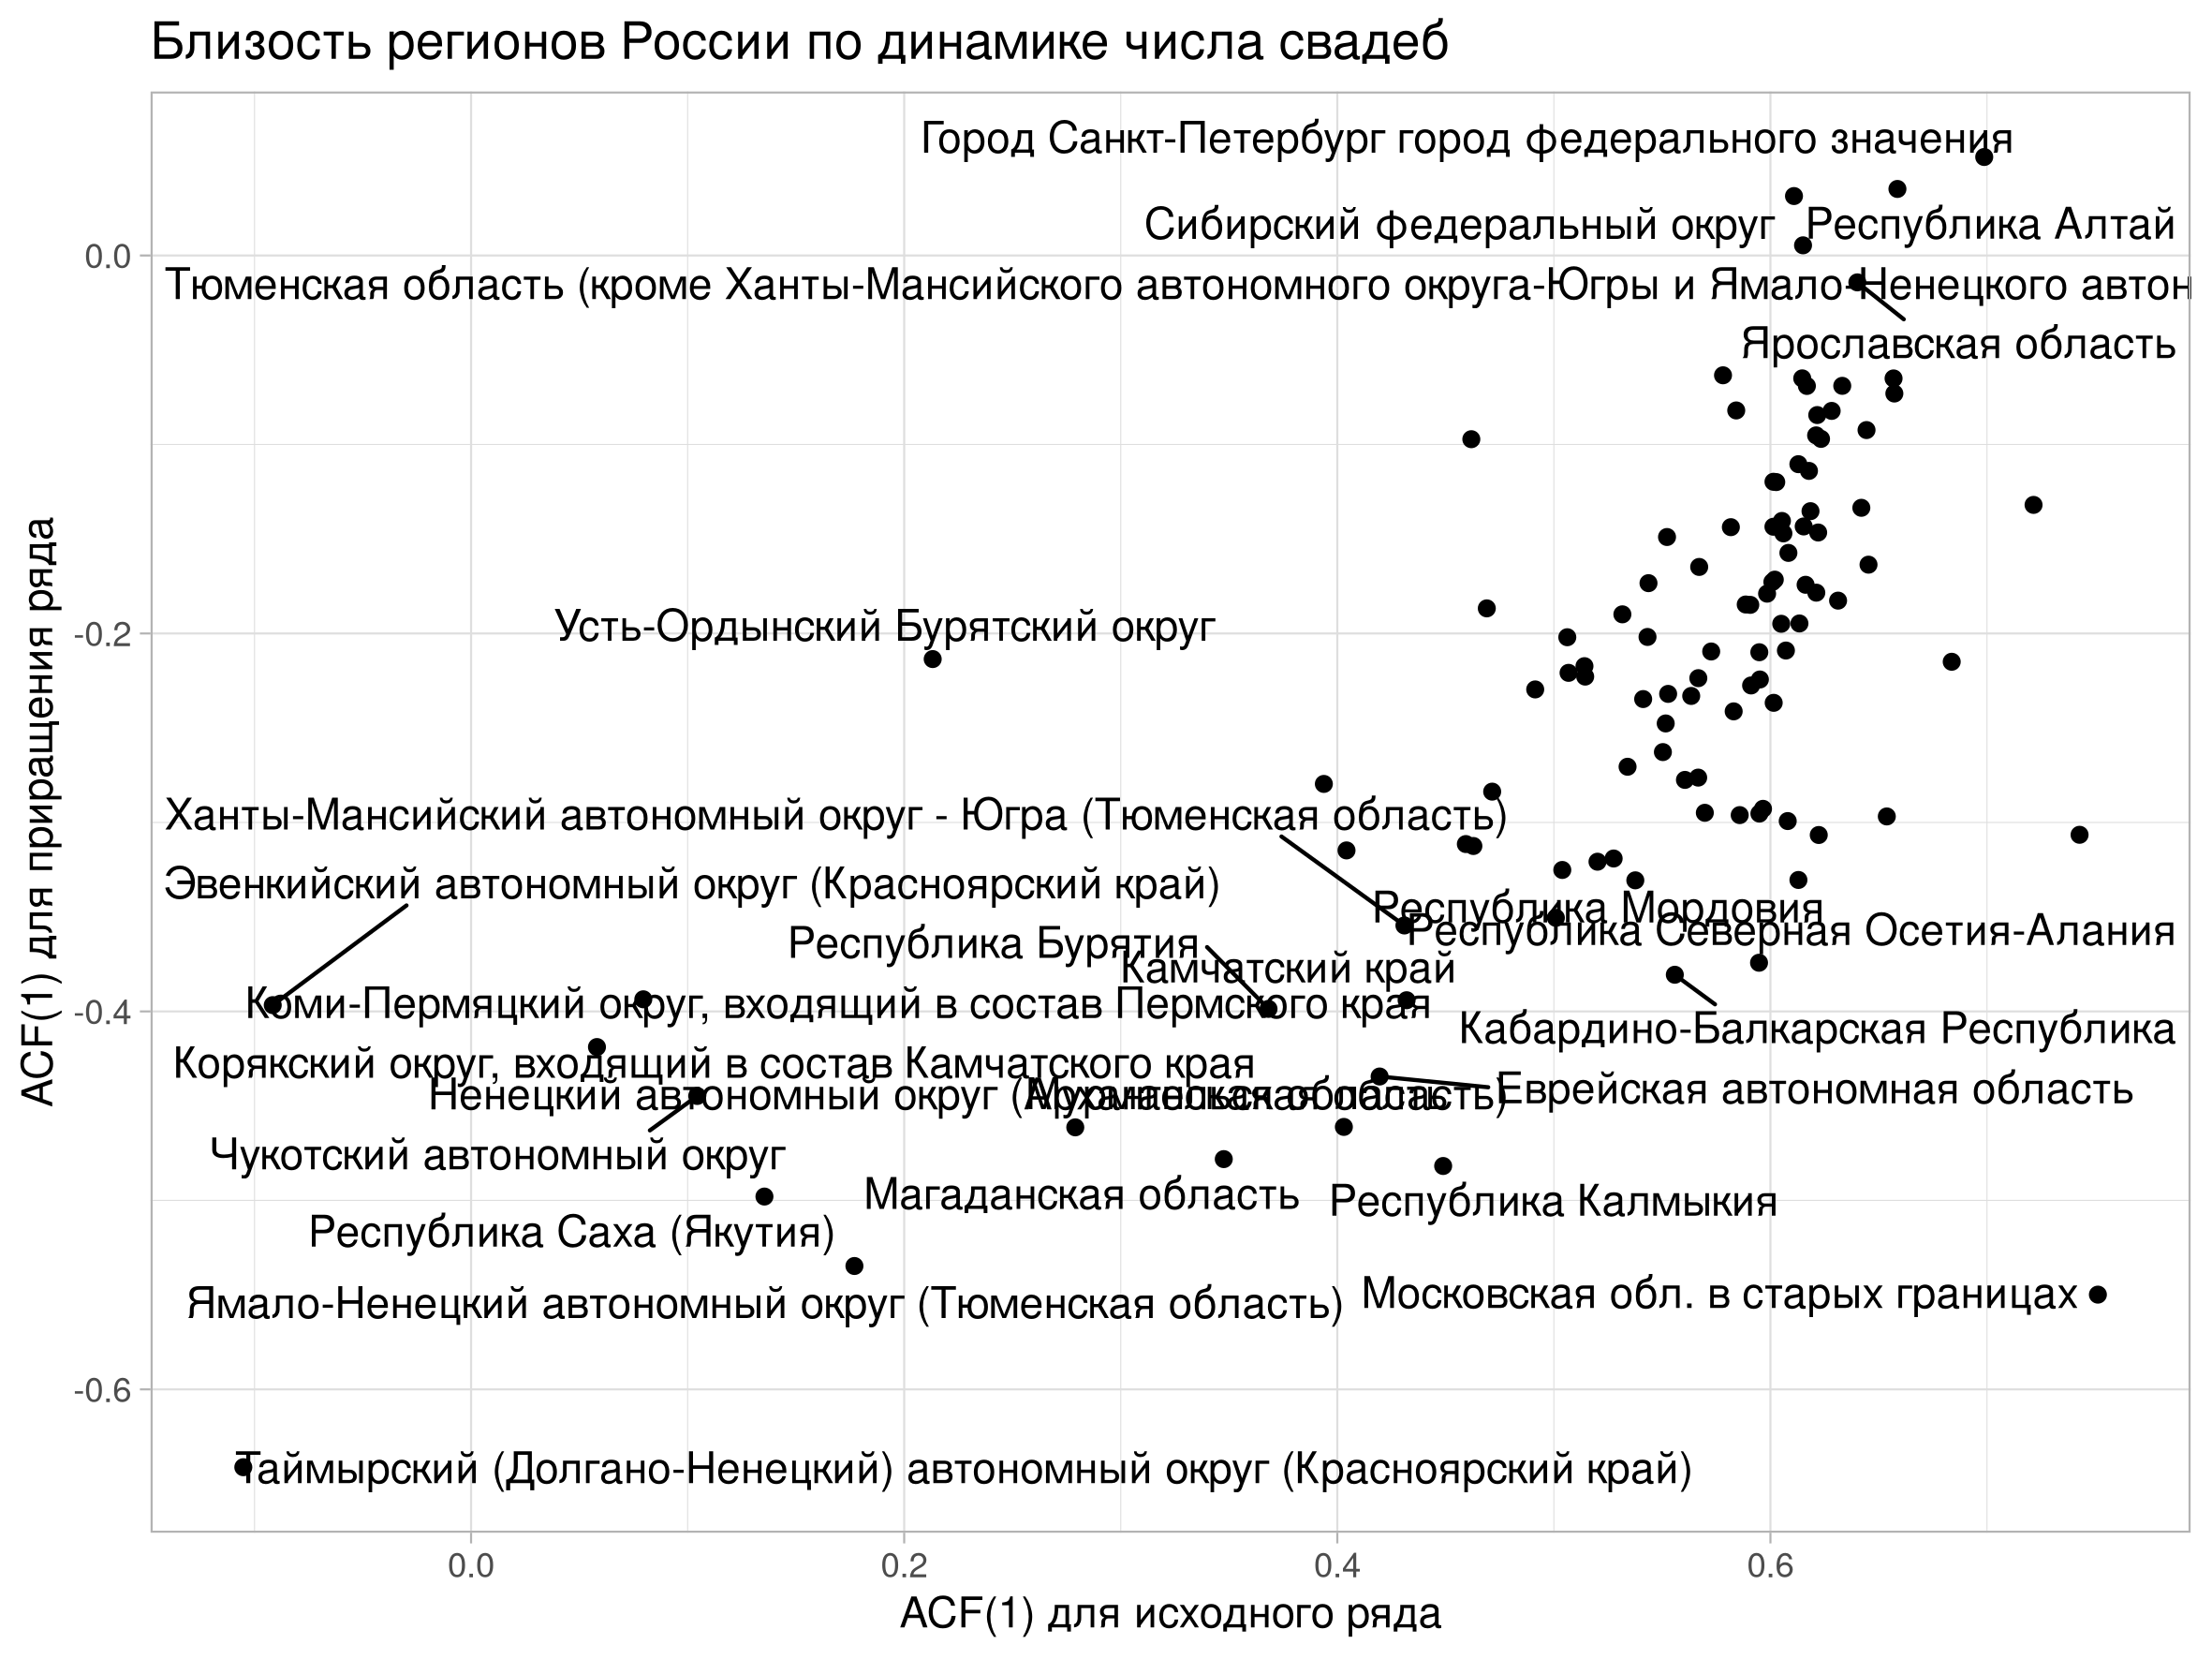
\includegraphics[width=\textwidth]{pictures/om_ts_01-025.png}


\end{frame}



\begin{frame}{Модели и алгоритмы}

\begin{block}{Модели}
\begin{itemize}[<+->]
  \item Явные предположения про величины $y_1$, $y_2$, \ldots, $y_T$.
  \item Метод оценивания: максимальное правдоподобие, байесовский подход.
  \item Точечные и интервальные прогнозы, проверка гипотез. 
\end{itemize}
\end{block}

ETS, ARIMA, ORBIT, PROPHET, \ldots

\end{frame}

\begin{frame}{Модели и алгоритмы}

\begin{block}{Алгоритмы}
  \begin{itemize}[<+->]
    \item Размытые предположения про величины $y_1$, $y_2$, \ldots, $y_T$.
    \item Особая инструкция.
    \item Точечные результаты без доверительных интервалов. 
  \end{itemize}
\end{block}
  
STL, градиентный бустинг, случайный лес, \ldots

\end{frame}

\begin{frame}{Фокус курса}

Прогнозирование одномерных рядов с помощью моделей. 

\end{frame}





% !TEX root = ../om_ts_01.tex

\begin{frame} % название фрагмента

\videotitle{Компоненты ряда}

\end{frame}



\begin{frame}{Компоненты ряда: план}
  \begin{itemize}[<+->]
    \item Тренд, цикличность и сезонность.
    \item Аддитивное и мультипликативное разложение.
    \item Откуда взять формальное определение?
  \end{itemize}

\end{frame}


\begin{frame}{Умение видеть единорогов}

Аддитивное разложение ряда:
\[
y_t = trend_t + seas_t + remainder_t.
\]

\pause

\alert{Тренд} — плавно изменяющаяся составляющая ряда.

\pause

\alert{Сезонная составляющая} — составляющая с чёткой периодичностью и стабильной интенсивностью.

\pause

\alert{Случайная компонента} (остаток) — всё остальное. 

\end{frame}

\begin{frame}{Тренд, сезонность и остаток}

  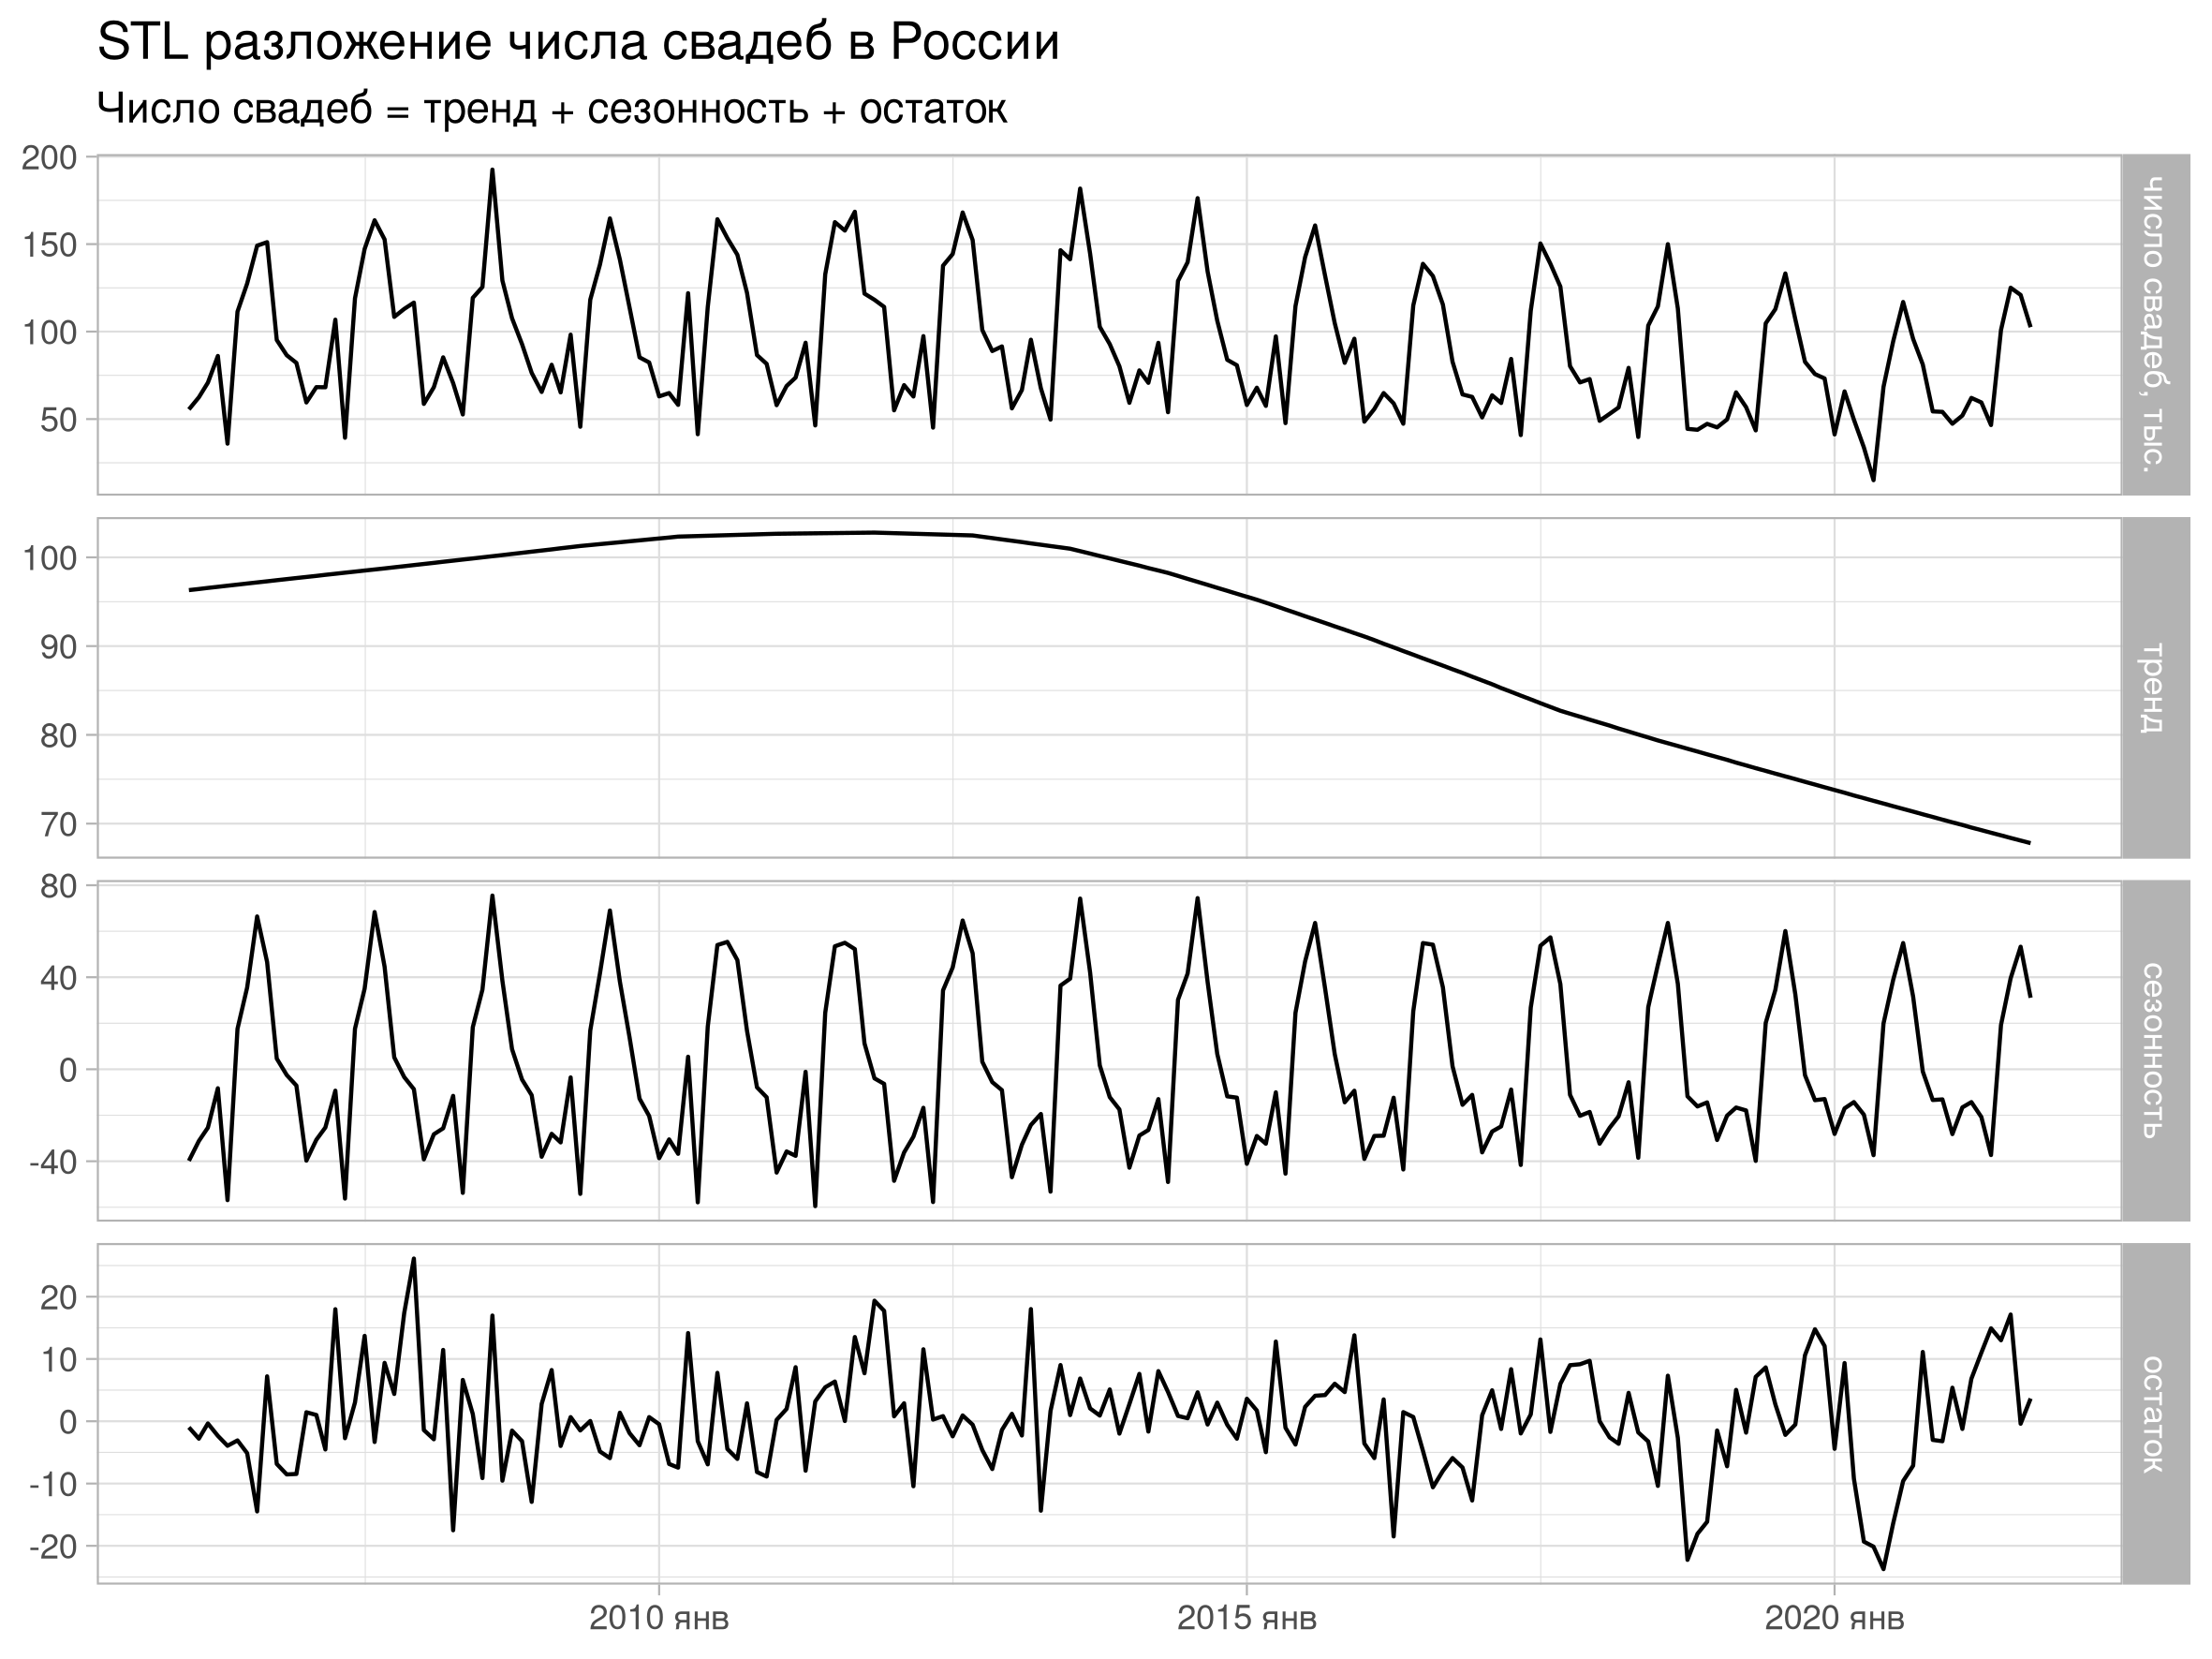
\includegraphics[width=\textwidth]{pictures/om_ts_01-041.png}

\end{frame}

\begin{frame}{Строгое определение?}

\pause
Единого строгого определения \alert{не} будет!

\pause
Некоторые модели и алгоритмы формально \alert{определяют} данные составляющие.

\end{frame}

\begin{frame}{Циклическая составляющая}

Иногда ряд раскладывают дальше
\[
y_t = trend_t + cycle_t + seas_t + remainder_t
\]

\pause
\alert{Циклическая составляющая} — составляющая с плавающей периодичностью и нестабильной интенсивностью. 


\pause
\alert{Тренд} (в узком смысле) —  плавно изменяющаяся монотонная составляющая ряда.

\end{frame}


\begin{frame}{Аддитивное и мультипликативное разложение}


\alert{Аддитивное} разложение ряда:
  \[
  y_t = trend_t + seas_t + remainder_t.
  \]
  
\pause
\alert{Мультипликативное} разложение ряда:
  \[
  y_t = trend_t \cdot seas_t \cdot remainder_t.
  \]

\pause
Превращаем одно в другое:
\[
  \ln y_t = \ln trend_t + \ln seas_t + \ln remainder_t.
\]
\end{frame}


\begin{frame}{Какие единороги лучше?}

Формальное определение составляющих \alert{зависит от модели}.

\pause
\alert{Алгоритм STL}: одно разложение $y_t = trend_t + seas_t + remainder_t$.

\pause
\alert{Модель ETS(AAA)}: другое разложение $y_t = trend_t + seas_t + remainder_t$.


\pause
Важно понимать \alert{цель построения} разложения. 

\end{frame}

\begin{frame}{А зачем разложение?}

  \begin{itemize}[<+->]
    \item Интересно \alert{само по себе}. 
    \item Для \alert{прогнозирования} ряда с помощью прогнозирования составляющих.
    \item Для получения \alert{характеристик ряда}. 
  \end{itemize}

  \pause
  А характеристики зачем?

  \begin{itemize}[<+->]
    \item Чтобы классифицировать новый ряд в один из заданных классов.
    \item Чтобы выявить в рядах неизвестные кластеры. 
  \end{itemize}
  
\end{frame}


\begin{frame}{Компоненты ряда: итоги}
  \begin{itemize}[<+->]
    \item Тренд \alert{плавно меняется} и включает цикличную составляющую.
    \item Сезонная составляющаю имеет \alert{чёткую периодичность} и \alert{стабильную амплитуду}.
    \item Точная формализация компонент \alert{зависит от модели}. 
  \end{itemize}

\end{frame}


% !TEX root = ../om_ts_01.tex

\begin{frame} % название фрагмента

\videotitle{Алгоритм STL}

\end{frame}



\begin{frame}{Алгоритм STL: план}
  \begin{itemize}[<+->]
    \item Локальная регрессия.
    \item Внешний цикл STL.
    \item Внутренний цикл STL.
    \item Параметры STL.
  \end{itemize}

\end{frame}


\begin{frame}{STL}

  \alert{STL} — Seasonal Trend decompositon with Loess.
  
  STL — разложение на сезонность и тренд с использованием LOESS.
  
  \pause
  
  \alert{LOESS} — LOcal regrESSion.
  
  LOESS — локальная линейная регрессия. 
  
\end{frame}


\begin{frame}{STL как чёрный ящик}

\alert{На входе:}

Ряд $Y_t$.

Параметры алгоритма $n_p$, $n_i$, $n_o$, $n_l$, $n_s$, $n_t$.

\pause
\alert{На выходе:}

Разложение $Y_t = T_t + S_t + R_t$.

\pause

Чёрный ящик \alert{долго} настраивали. 

\end{frame}


\begin{frame}{STL: результат}

  здесь будет картинка

\end{frame}

\begin{frame}{LOESS}

\begin{itemize}
  \item Хотим построить прогноз для точки $x$.
  \item Находим \alert{локальные оценки} $\hat\beta_1(x)$, $\hat\beta_2(x)$. 
  \[
      \min \sum_i \alert{K_h(x_i - x}) (y_i - \hat\beta_1 - \hat\beta_2 x_i)^2
  \]
  \item Прогнозируем:
  \[
  \hat y = \hat\beta_1(x) + \hat\beta_2(x) x.  
  \] 
\end{itemize}

\pause
\alert{Ядерная функция}
\begin{itemize}
  \item Функция $K_h(x_i - x)$ убывает с увеличением расстояния $|x_i - x|$;
  \item Параметр $h$ отвечает за ширину окна сглаживания. 
\end{itemize}

\pause
Например, $h$ — количество точек $x_i$ рядом с $x$, которые мы учитываем.

\end{frame}

\begin{frame}{Нюансы локальной регрессии}

  \begin{itemize}
    \item Выбор \alert{степени полинома}.
    \[
      \min \sum_i \alert{w_q(x_i - x}) (y_i - \hat\beta_1 - \hat\beta_2 x_i - \hat\beta_3 x_i^2)^2
    \]  
    \item Выбор \alert{ядерной} функции.
    \[
      w_h(d) = \frac{1}{\sqrt{2\pi}h} \exp(- d^2/2h^2)
    \]
    \item Выбор \alert{ширины окна} $h$.

\end{itemize}

\end{frame}

\begin{frame}{STL с высоты птичьего полёта}

Цель: разложение $Y_t = T_t + S_t + R_t$.

Алгоритм содержит два цикла: \alert{внешний} и \alert{внутренний}.

\begin{enumerate}[<+->]

  \item Инициализируем $T_t = 0$, $R_t = 0$.
  
  \alert{Внешний} цикл:

  \item Посчитаем вес каждого наблюдения, $\rho_t$. 

  На первом проходе $\rho_t = 1$ у каждого наблюдения. 

  На последующих проходах $\rho_t$ отрицательно зависит от свежей величины $R_t$.

  \item Обновим текущее разложение $Y_t = T_t + S_t + R_t$ с учётом весов $\rho_t$.
\end{enumerate}

\end{frame}



\begin{frame}{STL: внутренний цикл}

  Цель: обновить разложение $Y_t = T_t + S_t + R_t$.
  
  \begin{enumerate}[<+->]
  
    \item[1.] Удалим из ряда ранее посчитанный тренд:
    \[
      Y_t^{det} = Y_t - T_t.
    \]
    
    \item[2.] Разобъём детрендированный ряд на 12 подрядов. 
    
    \item[3.] Сгладим каждый подряд по отдельности с помощью LOESS:
    \[
    C^{jan} = LOESS_{\rho}(Y^{det}_{jan}), C^{feb} = LOESS_{\rho}(Y^{det}_{feb}), \ldots
    \]

    \item[4.] Выделяем низкочастотную составляющую (дважды скользящее среднее + LOESS):
    \[
    L_t = LOESS(MA(MA(C_t)))
    \]    
    \item[5-6.] Получаем новые $S_t^{new}$ и $T_t^{new}$.
  \end{enumerate}
  
  
  \end{frame}
  


  \begin{frame}{STL: внутренний цикл}
    
    \begin{enumerate}[<+->]
    
      \item[1-3.] Удалим из ряда ранее посчитанный тренд, разобъём на подряды и 
      сгладим каждый подряд с помощью LOESS. 
      
      \item[4.] Выделяем низкочастотную составляющую.
      \item[5.] Удаляем низкочастотную составляющую, получаем \alert{новую} сезонную компоненту:
      \[
      S_t^{new} = C_t - L_t.  
      \]
      \item[6.] Удаляем новую сезонность из исходного ряда и сглаживаем с помощью LOESS:
      \[
      T_t^{new} = LOESS_{\rho}(Y_t - S_t^{new}).
      \]
      
    \end{enumerate}
    
    
    \end{frame}
    
  
    \begin{frame}

      \begin{center}
        Уф!
      \end{center}

    \end{frame}
  

\begin{frame}{Параметры STL}

  \begin{itemize}[<+->]
    \item $n_p$ — периодичность сезонности, например, $n_p=12$.
    \item $n_o$ — число проходов внешнего цикла. 
    
    Чем больше число $n_o$, тем слабее влияние выбросов.

    Значение $n_o = 1$ часто достаточно.
    \item $n_i$ — число проходов внутреннего цикла. 

    Значение $n_o = 2$ часто достаточно для достижения сходимости.
  \end{itemize}
    
\end{frame}

\begin{frame}{Параметры сглаживания STL}

\begin{itemize}[<+->]
\item $n_l$ — сила сглаживания низкочастотного фильтра. 

\item $n_s$ — сила сглаживания сезонных подрядов.
\item $n_t$ — сила сглаживания при выделении тренда на последнем шаге. 

\end{itemize}

\alert{Что настроить?}
\begin{enumerate}[<+->]
  \item Обязательно указать периодичность $n_p$.
  \item Возможно, поиграться с $n_s$.
\end{enumerate}

\end{frame}

\begin{frame}{STL: итоги}
  \begin{itemize}[<+->]
    \item LOESS — локальная регрессия.
    \item STL — хорошо проверенный временем алгоритм без модели.
    \item При желании можно поиграться с силами сглаживания.
  \end{itemize}

\end{frame}



\end{document}

% !TEX root = ../om_ts_01.tex

\begin{frame} % название фрагмента

\videotitle{Характеристики рядов}

\end{frame}



\begin{frame}{Характеристики рядов: план}
  \begin{itemize}[<+->]
    \item Выборочная автокорреляция. 
    \item Выборочная частная автокорреляция.
    \item STL-характеристики.
  \end{itemize}

\end{frame}

\begin{frame}{Задачи для множества рядов}
  \begin{itemize}
    \item Классифицировать новый ряд в один из существующих классов.
    \item Понять, какие ряды близки к друг другу.
    \item Кластеризовать ряды на неизвестное множество кластеров.
  \end{itemize}
  \pause
  \alert{Как решить?}
  \begin{enumerate}[<+->]
    \item Для каждого ряда сгенерировать \alert{признаки}. 
    \item К полученным признакам применить алгоритм для перекрестных данных.
 \end{enumerate}
 \pause
 Классифицировать: с помощью случайного леса.

 Измерить расстояние с помощью метрики Махаланобиса. 

 Кластеризовать с помощью иерархической кластеризации. 

\end{frame}


\begin{frame}{Создаём признаки}

Два \alert{множества} признаков:
\begin{itemize}[<+->]
  \item Выборочная ACF (\alert{автокорреляционная функция}, AutoCorrelation Function).
  \item Выборочная PACF (\alert{частная} автокорреляционная функция, Partial ACF).
\end{itemize}

\pause
Из \alert{одного} ряд получим:

$ACF_1$, $ACF_2$, $ACF_3$, \ldots

$PACF_1$, $PACF_2$, $PACF_3$, \ldots
\end{frame}


\begin{frame}{ACF}

\begin{block}{Выборочная ACF}
  Оценим множество парных регрессий:
  \[
  \hat y_t = \hat\beta_1 + \hat\beta_2 y_{t-1}, \quad ACF_1 = \hat\beta_2;
  \]
  \pause
  \[
    \hat y_t = \hat\beta_1 + \hat\beta_2 y_{t-2}, \quad ACF_2 = \hat\beta_2;
  \]
  \pause
  \[
    \hat y_t = \hat\beta_1 + \hat\beta_2 y_{t-k}, \quad ACF_k = \hat\beta_2;
  \]
\end{block}

\pause
\alert{Смысл}
$ACF_2$: на сколько единиц в среднем $y_t$ выше среднего, если $y_{t-2}$ выше среднего на одну единицу.

\end{frame}


\begin{frame}{Ряд и его ACF}

  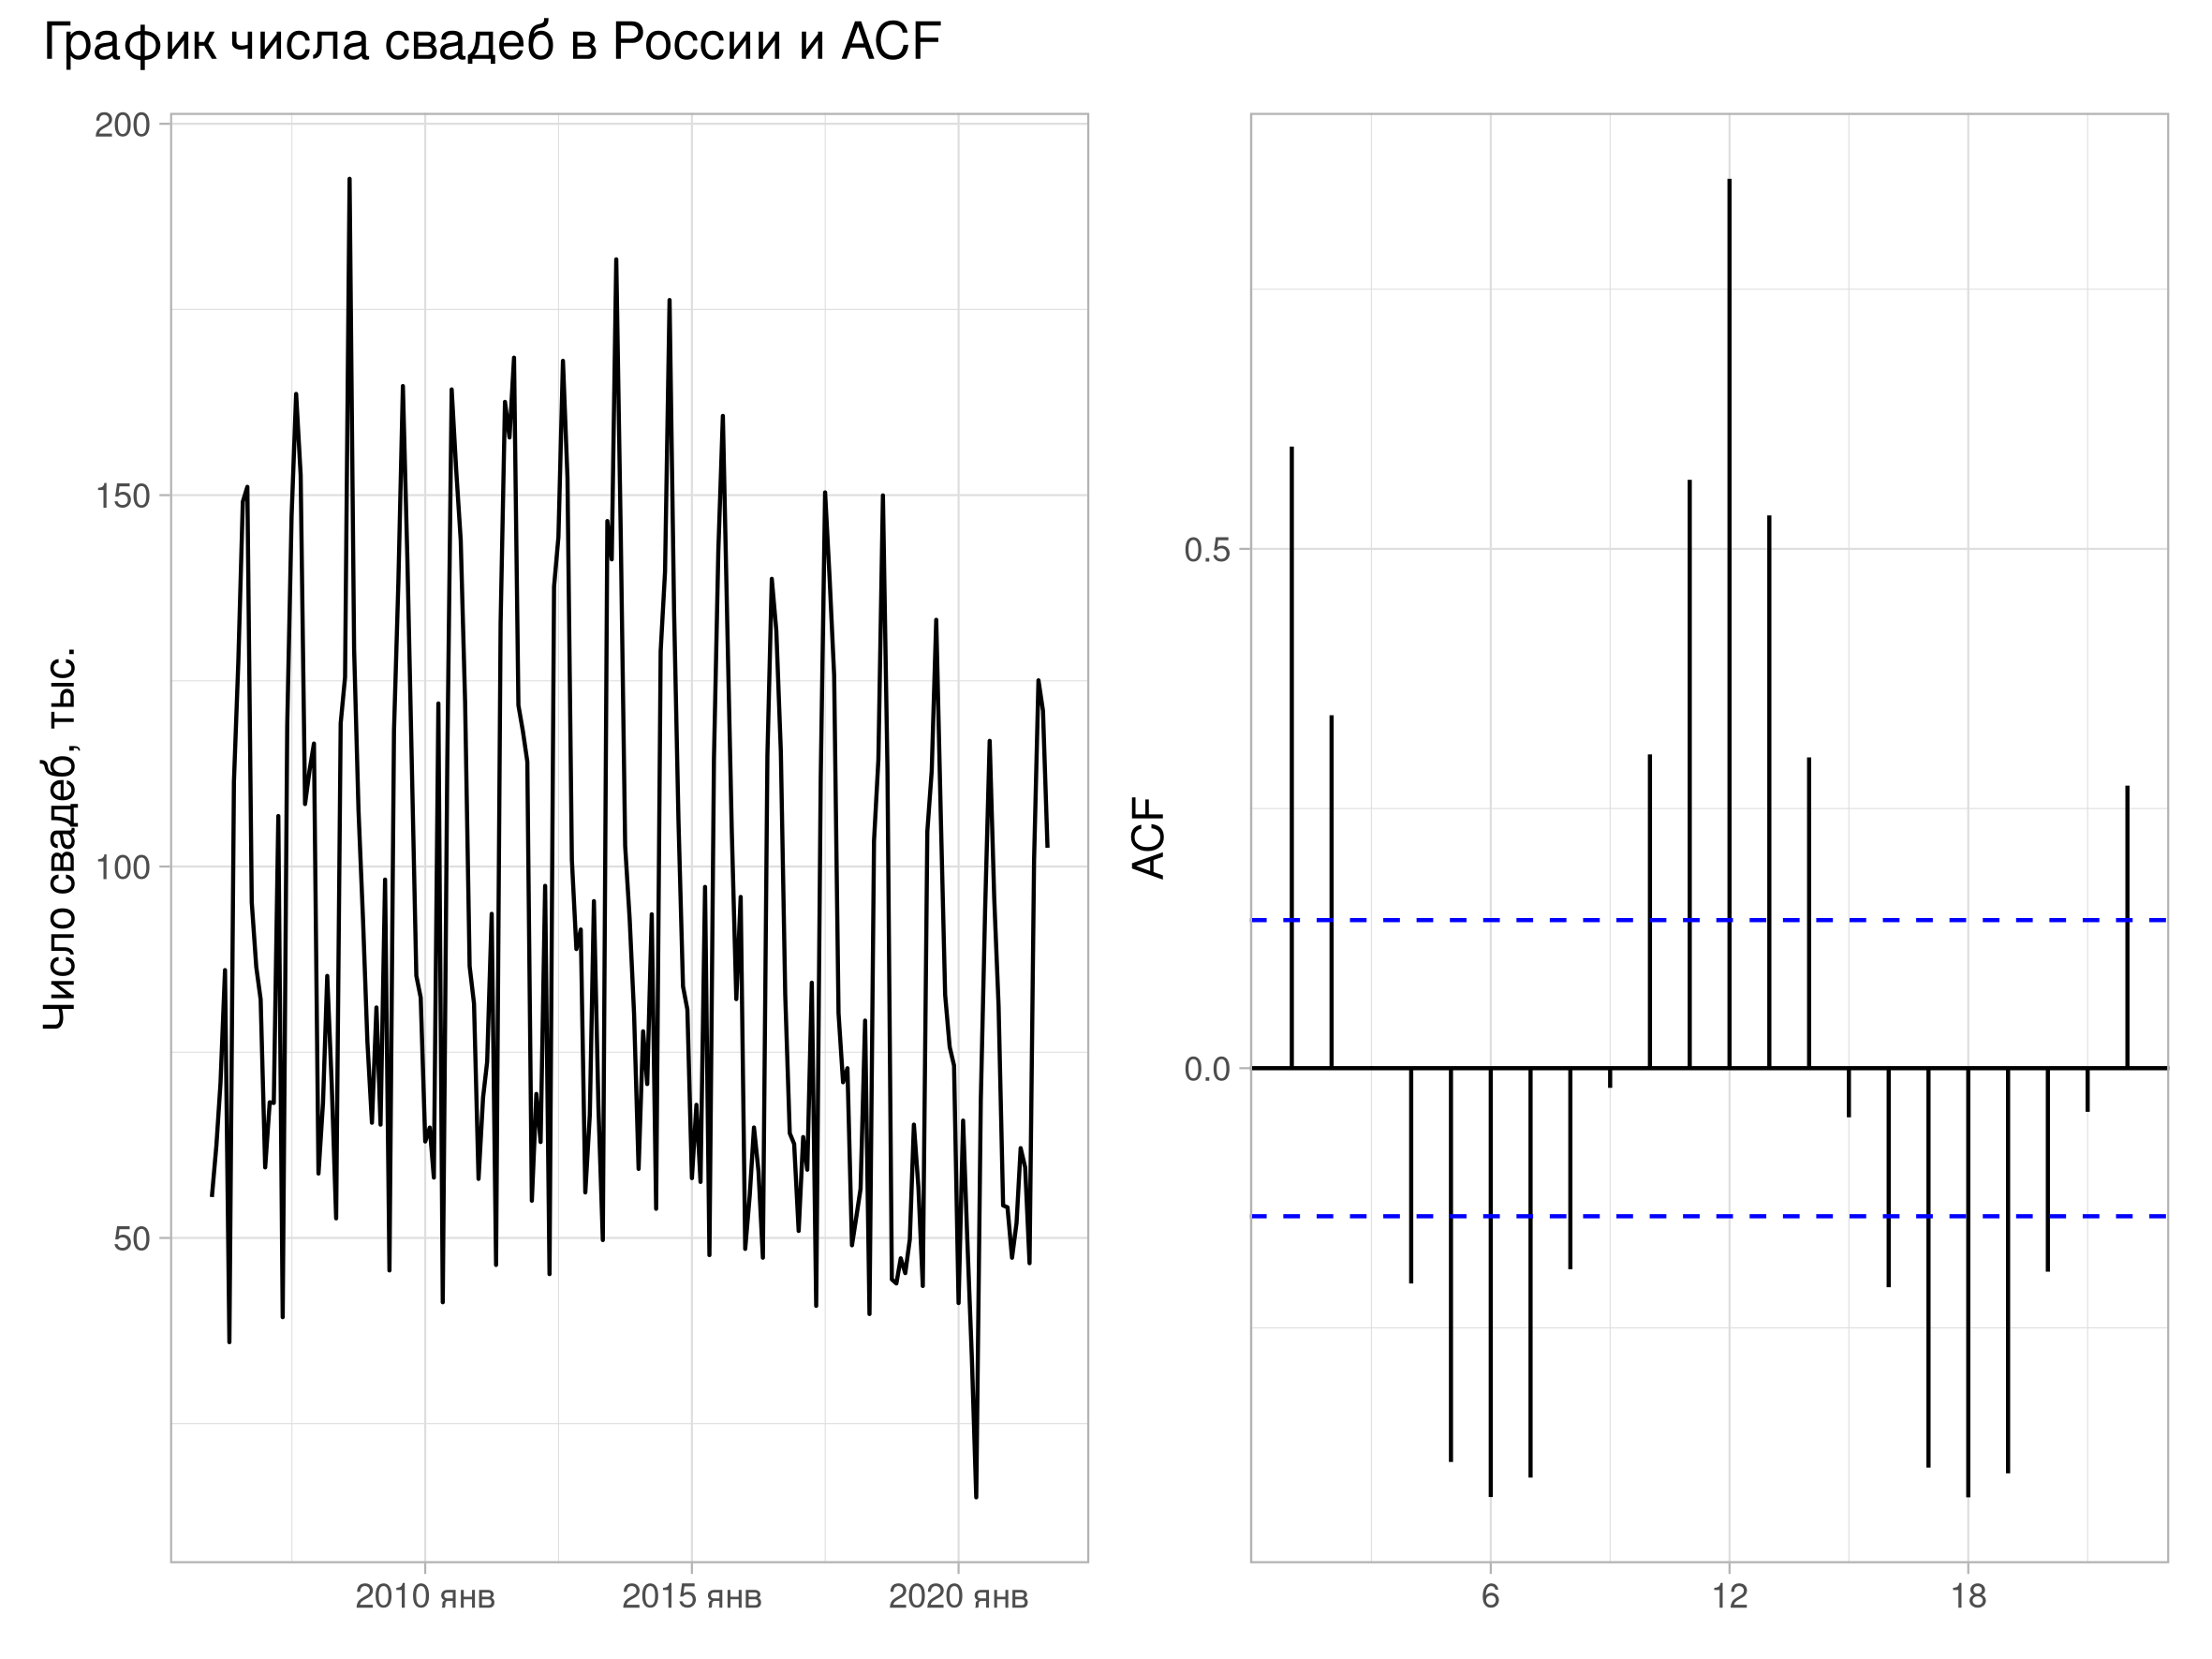
\includegraphics[width=\textwidth]{pictures/om_ts_01-120.png}

\end{frame}

\begin{frame}{Почему ACF — корреляция?}

  \alert{Классическое определение}

  \begin{block}{Выборочная ACF}
    $ACF_k$ — выборочная корреляция между рядом $y_t$ и рядом $y_{t-k}$.
  \end{block}

\pause
Различие между определениями \alert{мало}. 

\end{frame}


\begin{frame}{PACF}

  \begin{block}{Выборочная PACF}
    Оценим множество множественных регрессий:
    \[
    \hat y_t = \hat\alpha + \hat\beta_1 y_{t-1}, \quad PACF_1 = \hat\beta_1;
    \]
    \pause
    \[
      \hat y_t = \hat\alpha  + \hat\beta_1 y_{t-1} + \hat\beta_2 y_{t-2}, \quad PACF_2 = \hat\beta_2;
    \]
    \pause
    \[
      \hat y_t = \hat\alpha + \hat\beta_1 y_{t-1} + \ldots + \hat\beta_k y_{t-k}, \quad PACF_k = \hat\beta_k;
    \]
  \end{block}
  
  \pause
  \alert{Смысл}
  $PACF_2$: на сколько единиц в среднем $y_t$ выше среднего, если $y_{t-2}$ выше среднего на одну единицу,
  а $y_{t-1}$ на среднем уровне.

  \end{frame}
  
  \begin{frame}{Ряд и его PACF}

    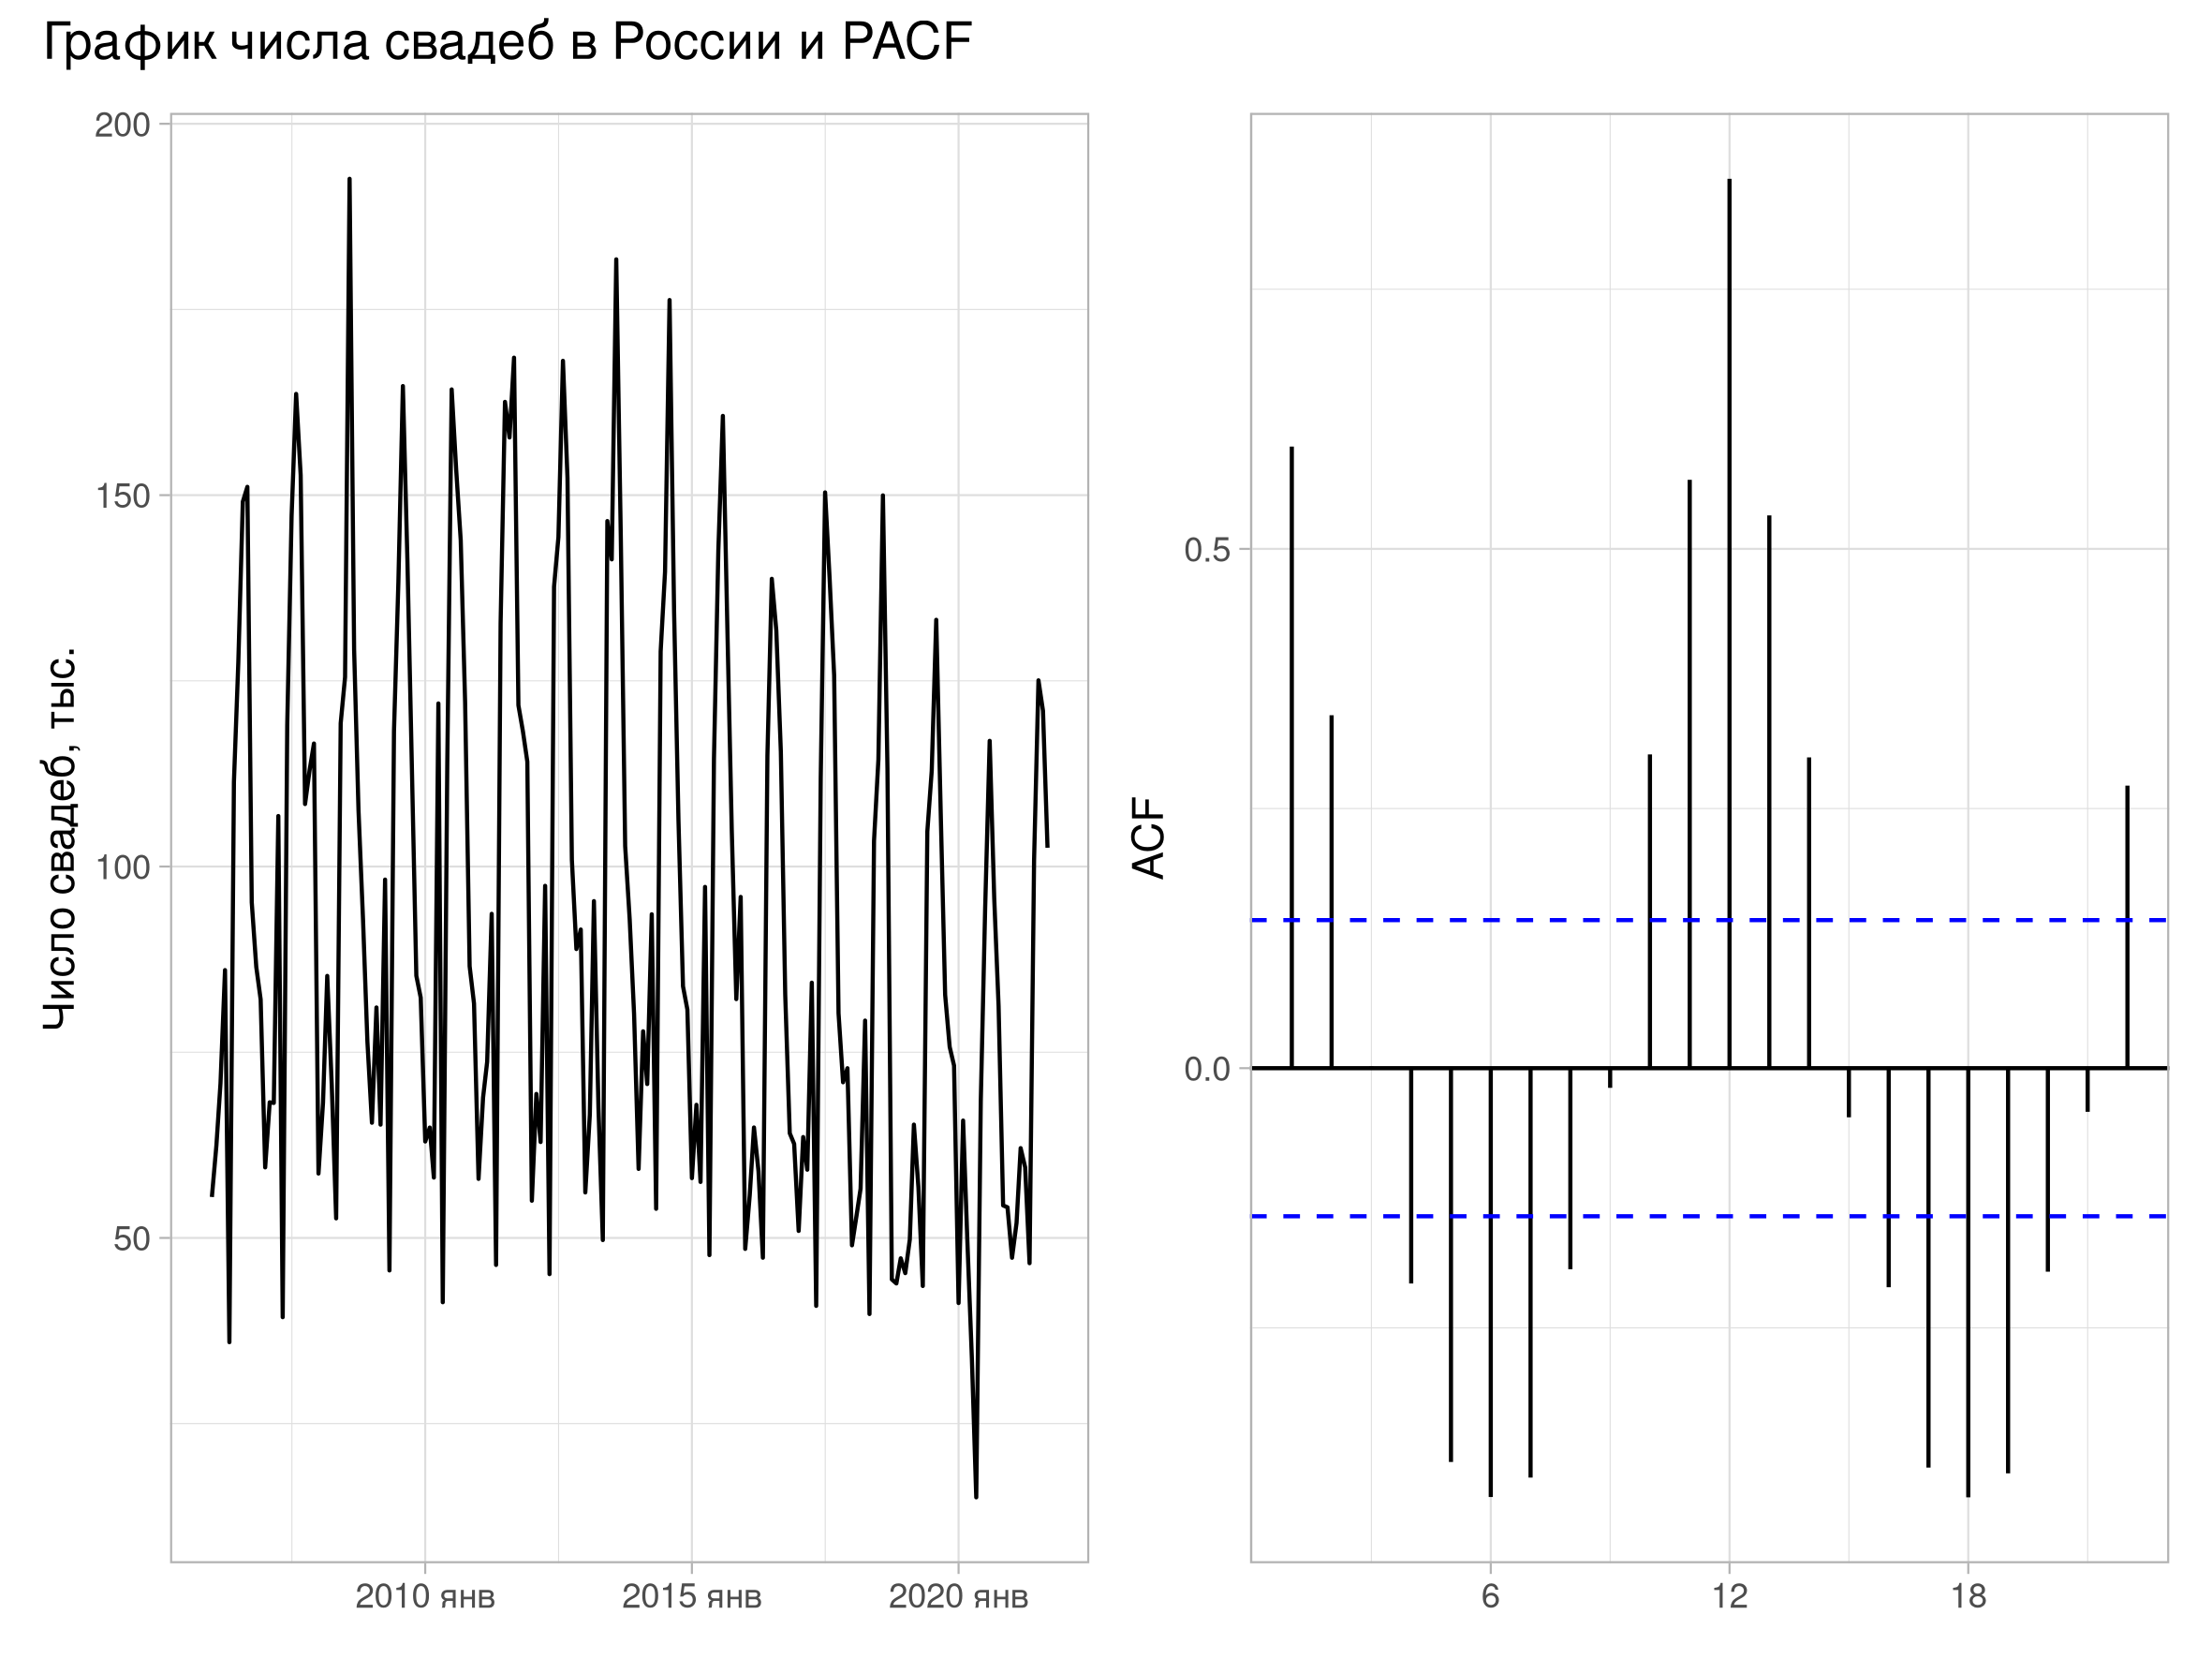
\includegraphics[width=\textwidth]{pictures/om_ts_01-127.png}
    
  \end{frame}
    
  \begin{frame}{Почему PACF — корреляция?}

    \alert{Классическое определение}
  
    \begin{block}{Выборочная PACF}
      $PACF_4$ — выборочная корреляция между остатками $a_t$ и остатками $b_t$.

      $a_t$ — остатки из регрессии
      \[
        y_t \text{ на } 1, y_{t-1}, y_{t-2}, y_{t-3}.
      \]

      $b_t$ — остатки из регрессии
      \[
        y_{t-4} \text{ на } 1, y_{t-1}, y_{t-2}, y_{t-3}.
      \]
    \end{block}
  
  \pause
  Различие между определениями \alert{мало}. 
  
  \end{frame}
  

  \begin{frame}{STL-характеристики}

    \alert{На выходе:}
    \[
      y_t = T_t + S_t + R_t.
    \]

    \pause
    Измерим:
    \begin{itemize}
      \item Выраженность тренда $F_{trend}$.
      \item Выраженность сезонности $F_{seas}$.
    \end{itemize}

  \end{frame}

  \begin{frame}{Выраженность тренда и сезонности}

    Получили разложение:
    \[
      y_t = trend_t + seas_t + remainder_t.
    \]
    
    \pause
    \alert{Идея определения:}
    При идеальном разложении с некоррелированными компонентами:
    \[
      F_{trend} = \frac{\sVar(trend)}{\sVar(trend) + \sVar(remainder)},
    \]

    \pause
    \[
    F_{seas} = \frac{\sVar(seas)}{\sVar(seas) + \sVar(remainder)},
  \]
  \end{frame}

  \begin{frame}{Выраженность тренда и сезонности}

    Получили разложение:
    \[
      y_t = trend_t + seas_t + remainder_t.
    \]

    \pause
    \alert{На практике}:
    \begin{itemize}[<+->]
      \item Выраженность тренда:
      \[
        F_{trend} = \max\left\{1 - \frac{\sVar(remainder)}{\sVar(trend + remainder)}, 0 \right\}.
      \]
      \item Выраженность сезонности:
      \[
        F_{seas} = \max\left\{1 - \frac{\sVar(remainder)}{\sVar(seas + remainder)}, 0 \right\}.
      \]

    \end{itemize}



  \end{frame}


  \begin{frame}{Выраженность тренда и сезонности}

    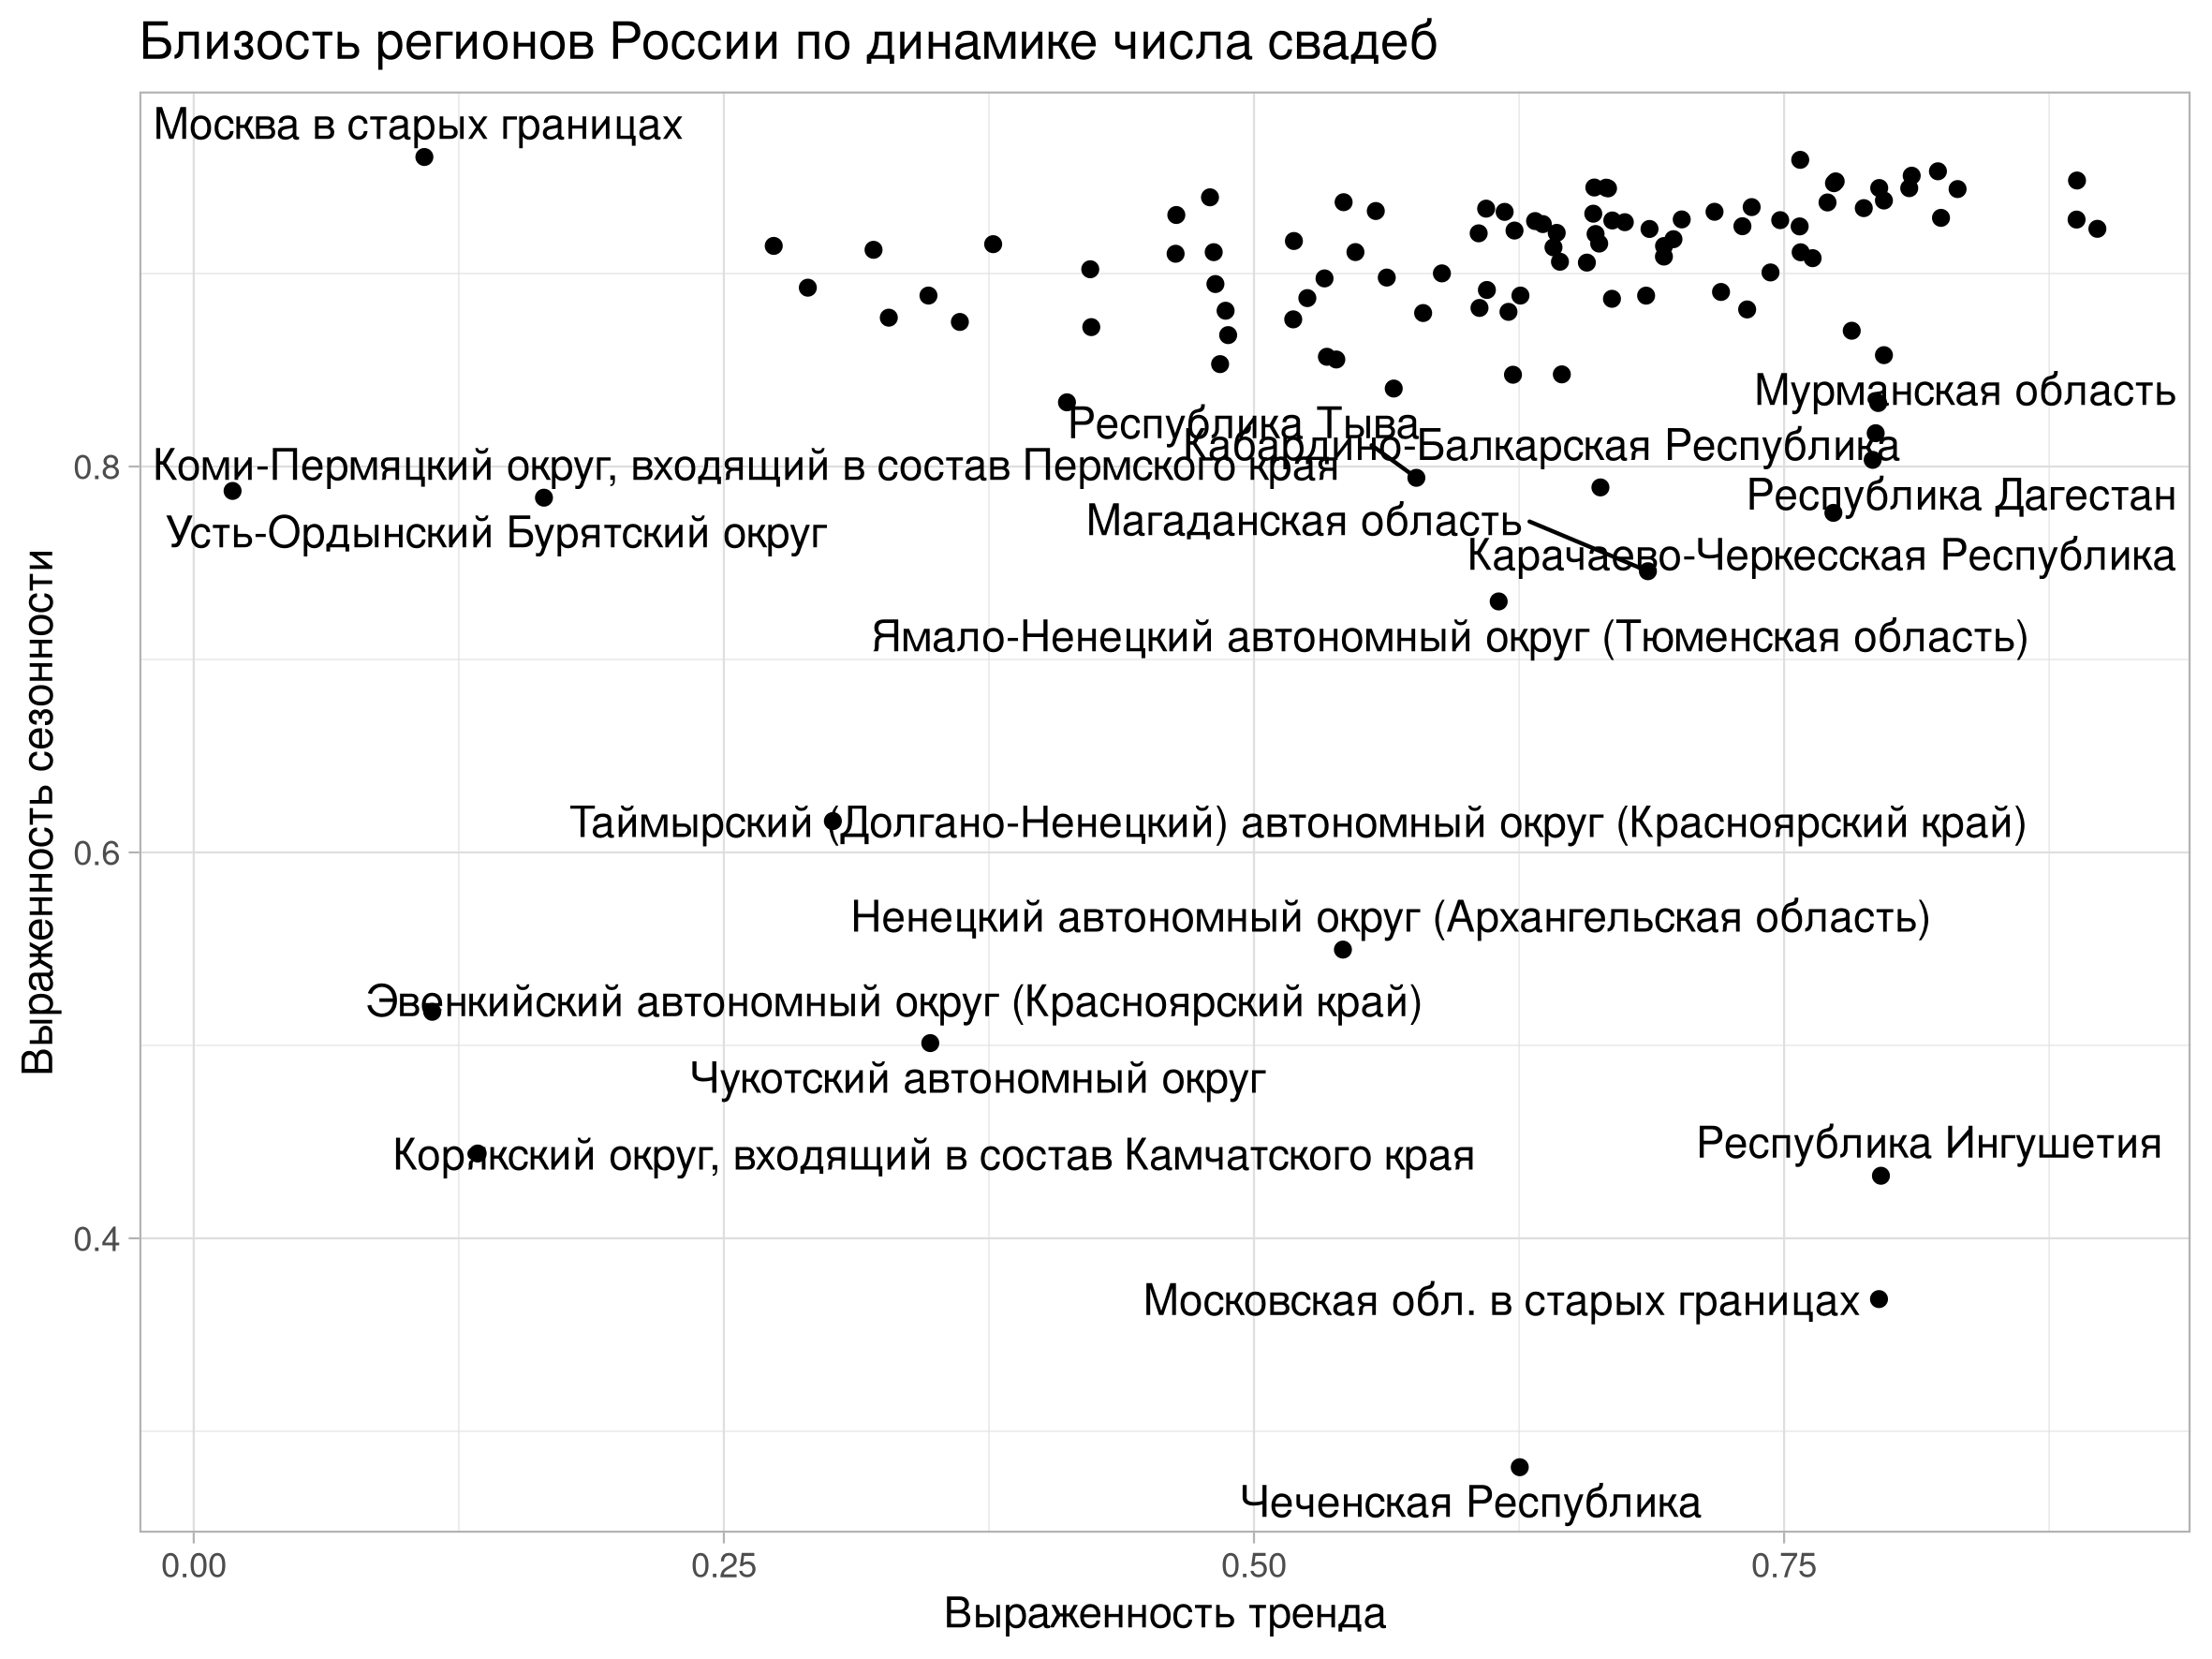
\includegraphics[width=\textwidth]{pictures/om_ts_01-138.png}

    
  \end{frame}
  


\begin{frame}{Характеристики рядов: итоги}

  \begin{itemize}[<+->]
    \item ACF — коэффициенты в \alert{парных} регрессиях или корреляции.
    \item PACF — коэффициенты во \alert{множественных} регрессиях или корреляции.
    \item STL позволяет измерить \alert{выраженность тренда и сезонности} по сравнению с остаточной компонентой.
  \end{itemize}
\end{frame}



% !TEX root = ../om_ts_01.tex

\begin{frame} % название фрагмента

\videotitle{Простейшие модели}

\end{frame}



\begin{frame}{Простейшие модели: план}
  \begin{itemize}[<+->]
    \item Белый шум. 
    \item Независимые наблюдения.
    \item Случайное блуждание.
  \end{itemize}

\end{frame}

\begin{frame}{Белый шум}

\begin{block}{Белый шум}
Временной ряд $u_t$ — белый шум, если:
\begin{itemize}
  \item $\E(u_t) = 0$;
  \item $\Var(u_t) = \sigma^2$;
  \item $\Cov(u_s, u_t) = 0$ при $s\neq t$.
\end{itemize}
\end{block}

\pause
\begin{itemize}[<+->]
  \item Составная часть всех моделей. Чаще всего белый шум — это, что отказались моделировать. 
  \item Часто дополнительно предполагают \alert{независимость} и \alert{нормальность}. 
  \item В белом шуме \alert{черти водятся}.
  
  ARCH, GARCH модели волатильности основаны на том, что $u_t$ и $u_s$ могут быть зависимы!
\end{itemize}

\end{frame}


\begin{frame}{Независимые наблюдения}

  \begin{block}{Модель}
  \[
  y_t = \mu + u_t,  
  \]
  где $u_t$ — белый шум, $u_t \sim \dN(0;\sigma^2)$.
  \end{block}
  \pause
  \alert{Оценки:}
  \[
  \hat \mu_{ML} = \bar y, \quad \hat\sigma^2_{ML} = \frac{\sum(y_i - \bar y)^2}{T}.  
  \]
  \pause
  \alert{Интервальный прогноз} на $h$ шагов вперёд:
  \[
  [\bar y - 1.96 \hat\sigma; \bar y + 1.96 \hat \sigma]  
  \]
\end{frame}
  

\begin{frame}{Случайное блуждание}

  \begin{block}{Наивная модель}
  \[
  y_t = y_{t-1} + u_t,  
  \]
  где $u_t$ — белый шум, $u_t \sim \dN(0;\sigma^2)$, задано стартовое $y_1$.
  \end{block}
  \pause
  Переформулируем: $y_t - y_{t-1} = \Delta y_t = u_t$.
  \pause
  \alert{Оценки:}
  \[
  \hat\sigma^2_{ML} = \frac{\sum(\Delta y_i - \overline {\Delta y})^2}{T - 1}.  
  \]
  \pause
  \alert{Интервальный прогноз} на $h$ шагов вперёд:
  \[
  [y_T - 1.96 \hat \sigma \sqrt{h}; y_T + 1.96 \hat \sigma  \sqrt{h}]  
  \]
\end{frame}

\begin{frame}{Первые прогнозы!}

  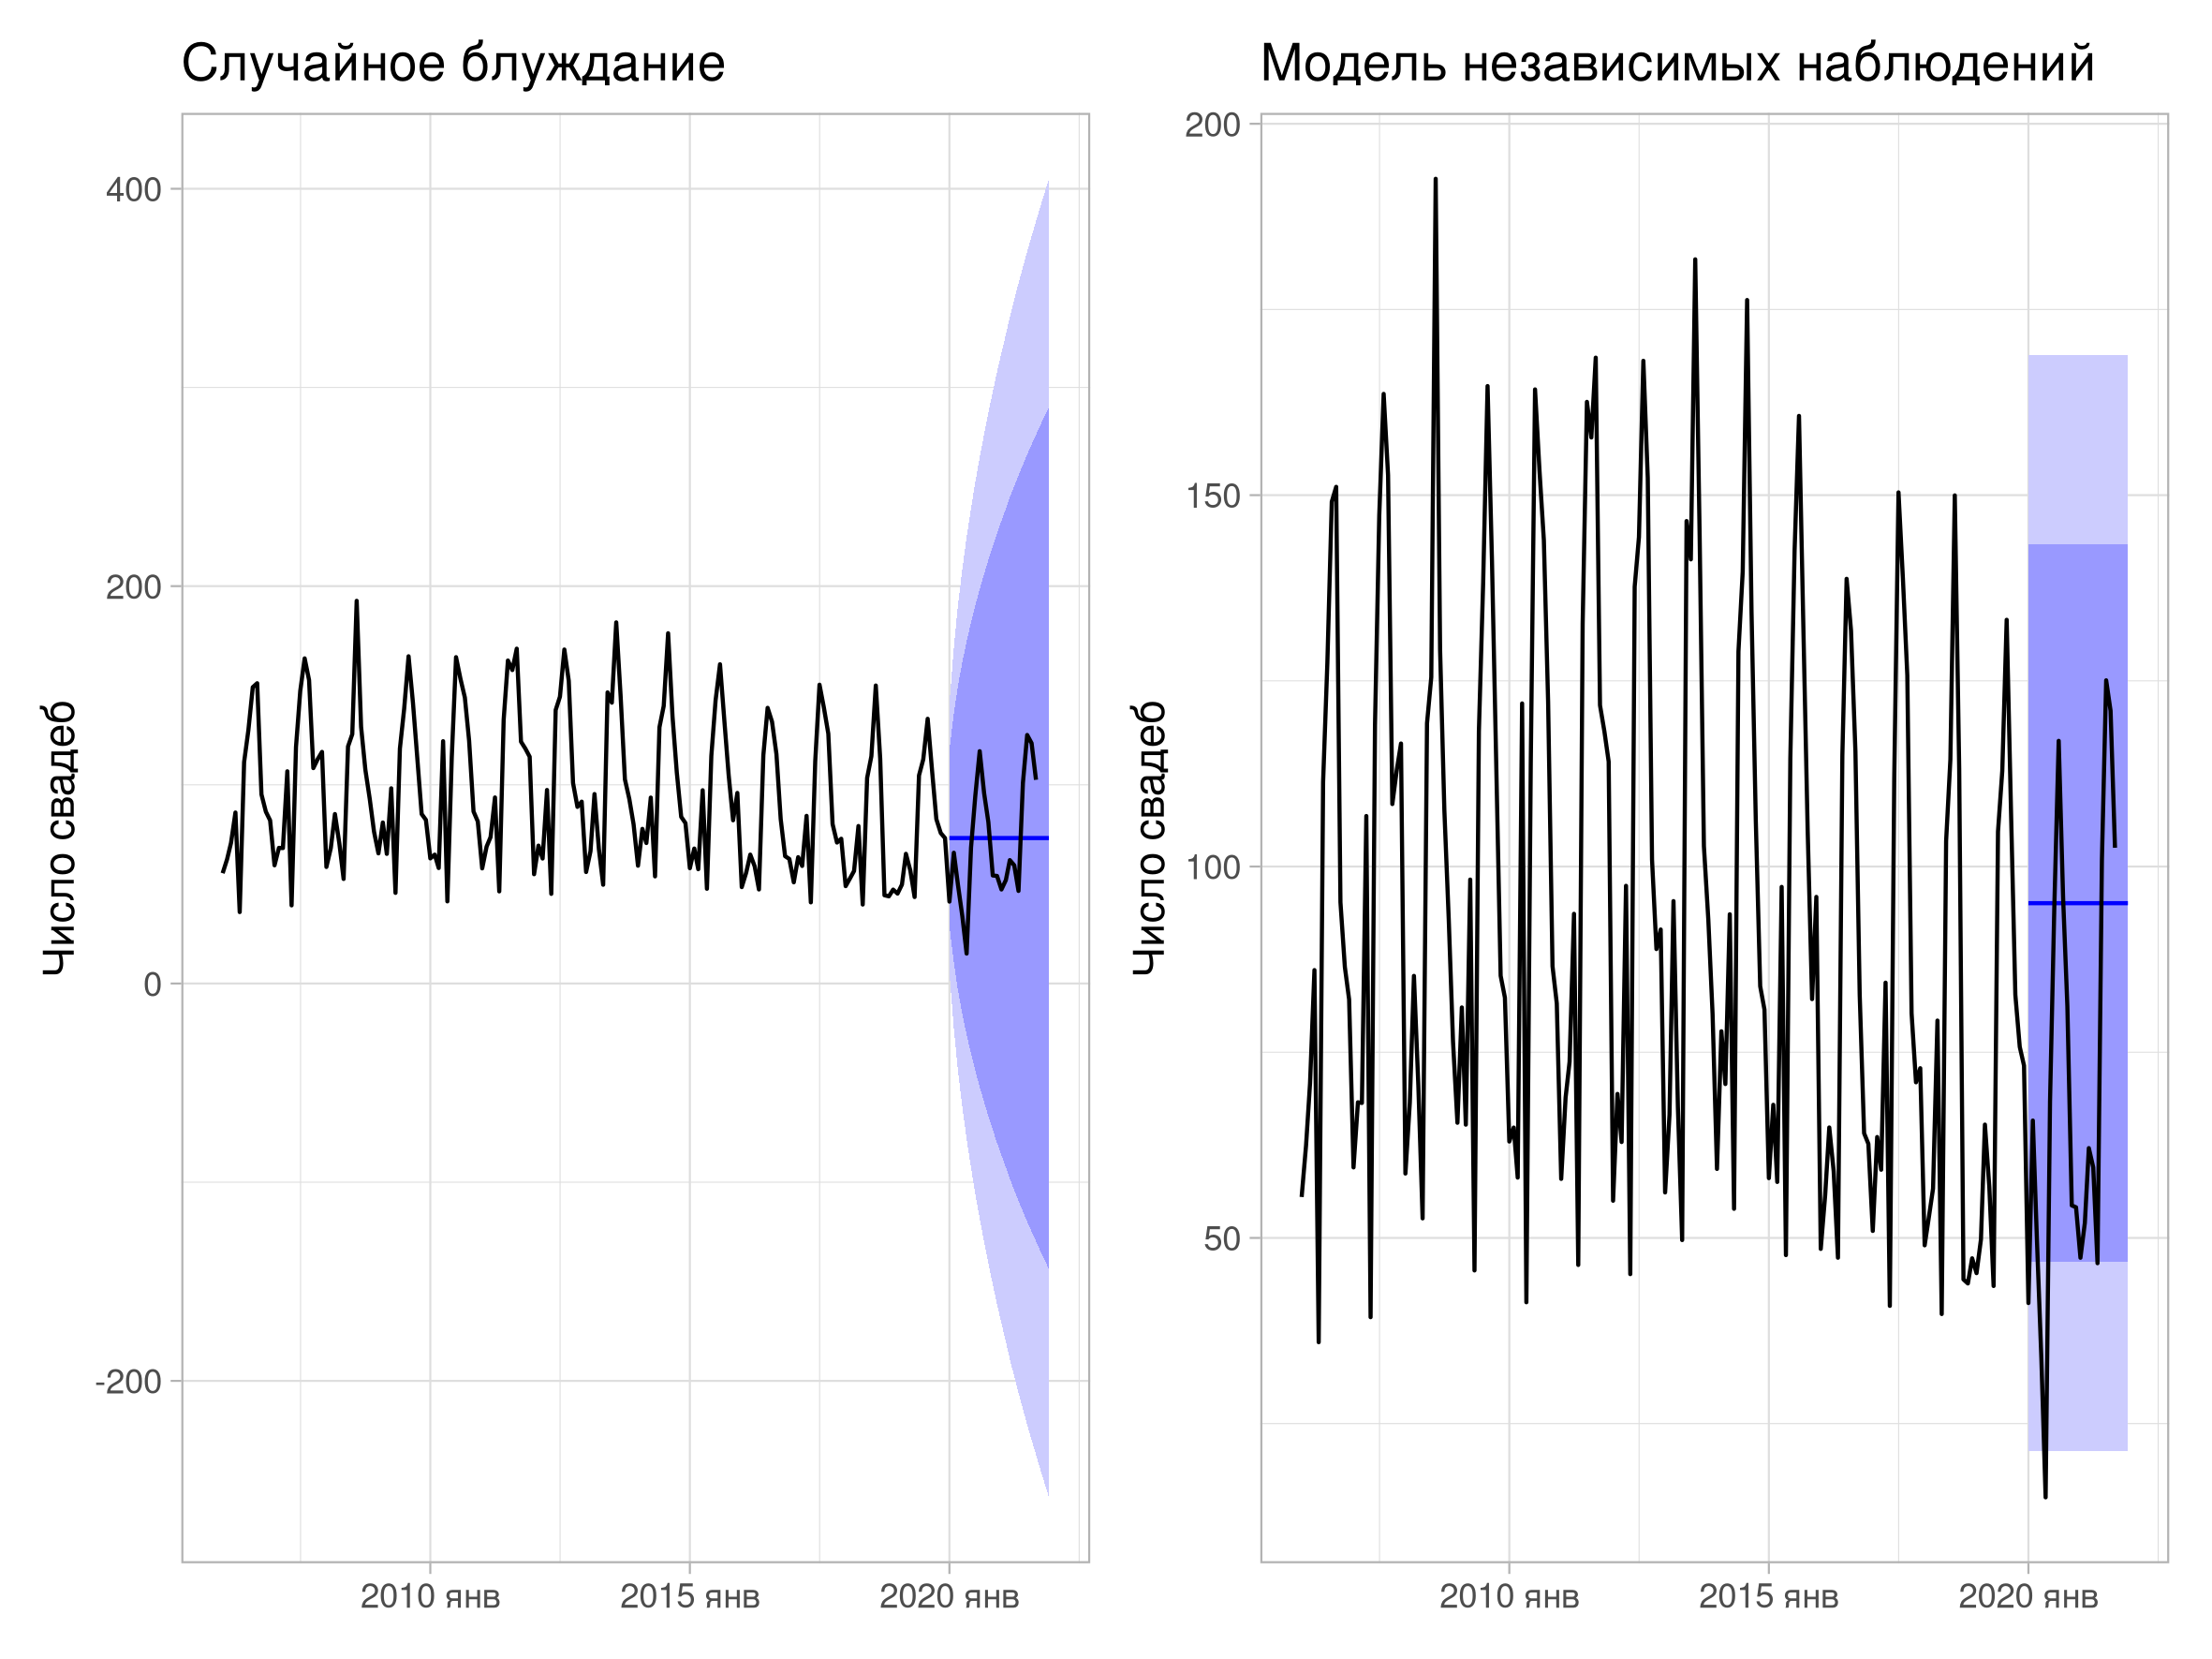
\includegraphics[width=\textwidth]{pictures/om_ts_01-157.png}

\end{frame}


\begin{frame}{Сезонное случайное блуждание}

  \begin{block}{Сезонная наивная модель}
  \[
  y_t = y_{t-12} + u_t,  
  \]
  где $u_t$ — белый шум, $u_t \sim \dN(0;\sigma^2)$, заданы $y_1$, \ldots, $y_{11}$.
  \end{block}
  \pause
  Переформулируем: $y_t - y_{t-12} = \Delta_{12} y_t = u_t$.
  \pause
  \alert{Оценки:}
  \[
  \hat\sigma^2_{ML} = \frac{\sum(\Delta_{12} y_i - \overline {\Delta_{12} y})^2}{T - 12}.  
  \]
  \pause
  \alert{Интервальный прогноз} на $h$ \alert{сезонов} вперёд:
  \[
  [y_{T} - 1.96 \hat \sigma \sqrt{h}; y_{T} + 1.96 \hat \sigma  \sqrt{h}]  
  \]
\end{frame}

\begin{frame}{Уже неплохо!}

  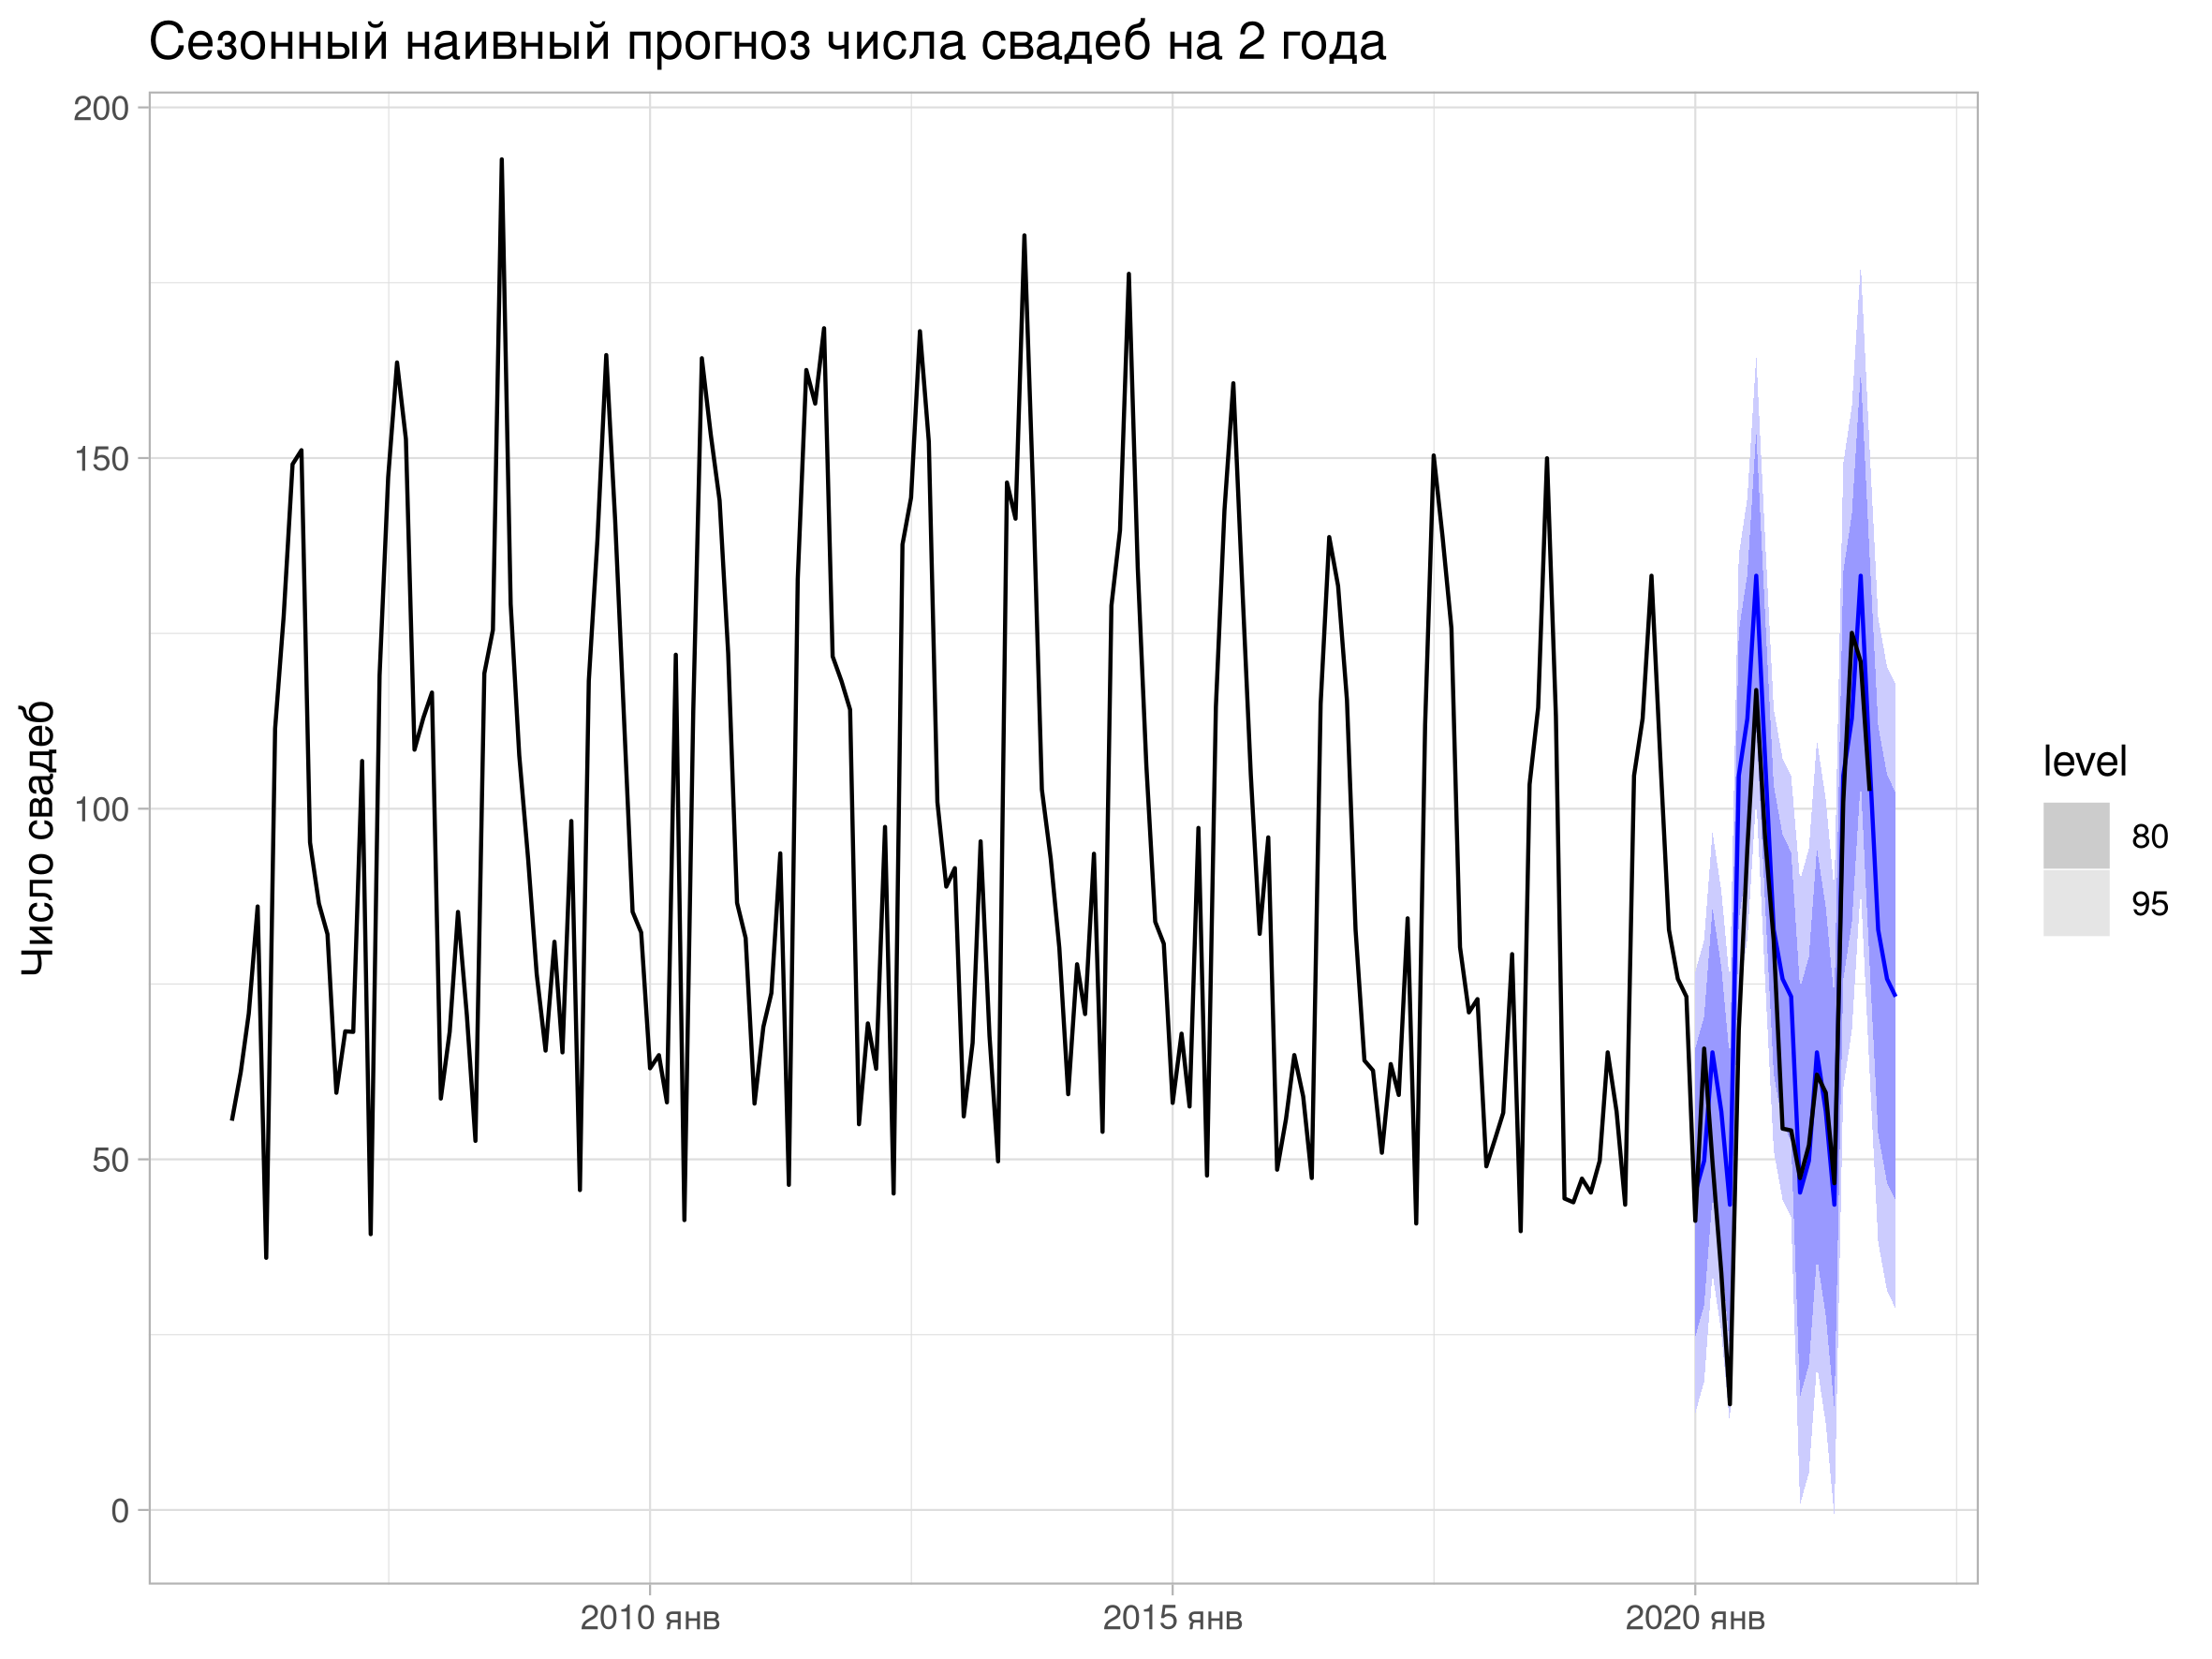
\includegraphics[width=\textwidth]{pictures/om_ts_01-162.png}


\end{frame}


\begin{frame}
  \frametitle{Зачем нужны наивные модели?}

  \begin{itemize}[<+->]
    \item \alert{Идеи} для сложных моделей.
    
    Модели \alert{стационарных рядов} похожи на модель независимых наблюдений. 

    Модели \alert{нестационарных рядов} похожи на случайное блуждание. 

    \item \alert{База для сравнения}. 
    
    При оценке сложной модели очень важно иметь базу сравнения. 

    \item \alert{Помощники} других моделей. 
    
    Можно \alert{усреднить прогнозы} сложной модели и наивной сезонной!
  \end{itemize}
  

\end{frame}

\begin{frame}{Наивные модели: итоги}

  \begin{itemize}[<+->]
    \item Белый шум — то, что не охота моделировать. 
    \item Независимые наблюдения и случайное блуждание.
    \item Идеи, составные части и помощники других моделей.
    \item База для сравнения.
  \end{itemize}
\end{frame}



\end{document}
